% ============================================================
%  The Particle Model — Lesson Booklet (one section per lesson: A Reading · B Theory · C Practice · D Above level)
%  Year 7 (Year 8 extension)  |  Victorian Curriculum F–10 Version 2.0
%  Compile with: xelatex three times, then python3 fill.py Particle_Model_Lesson_Booklet_Yr7
% ============================================================
\documentclass[11pt,a5paper,twoside]{article}
\newcommand{\unitname}{Separation Technologies and Techniques}\newcommand{\unitcaps}{SEPARATION}

% ── Fonts (compile with LuaLaTeX) ────────────────────────────────────────────
\usepackage{fontspec}
% Bundled fonts (in ./fonts/) so the document compiles anywhere with XeLaTeX/LuaLaTeX
\setmainfont{Lato}[                   % body — humanist sans (stands in for deck's Inter)
  Path=../fonts/, Extension=.ttf, Ligatures=TeX,
  UprightFont=Lato-Regular, ItalicFont=Lato-Italic,
  BoldFont=Lato-Bold, BoldItalicFont=Lato-BoldItalic ]
\newfontfamily\headingfont{Poppins}[  % display/headings — matches the slide decks
  Path=../fonts/, Extension=.ttf, Ligatures=TeX,
  UprightFont=Poppins-Regular, ItalicFont=Poppins-Italic,
  BoldFont=Poppins-Bold, BoldItalicFont=Poppins-BoldItalic ]
\setlength{\headheight}{22pt}

\usepackage[protrusion=true,expansion=false]{microtype}
\usepackage[a5paper, inner=17mm, outer=13mm, top=19mm, bottom=17mm, headheight=14pt, headsep=4mm, footskip=8mm]{geometry}
\usepackage{xcolor}
\usepackage{tikz}
\usetikzlibrary{arrows.meta, shapes.geometric, calc, positioning, decorations.pathreplacing}
\usepackage{tcolorbox}
\tcbuselibrary{skins, breakable, raster}
\usepackage{fancyhdr}
\usepackage{titlesec}
\usepackage{enumitem}
\usepackage{booktabs}
\usepackage{tabularx}
\usepackage{array}
\usepackage{colortbl}
\usepackage{multicol}
\usepackage{amsmath}
\usepackage{needspace}
% TikZ diagram macros are embedded below (just before \begin{document}) for easy editing.
\usepackage{longtable}
\usepackage{graphicx}
\usepackage{lastpage}
\usepackage{calc}
\usepackage{mdframed}
\usepackage{setspace}
\usepackage{ragged2e}
% PDF bookmarks: one per lesson (made in \sectiondiv) plus the cover and
% contents, and links from the contents table to each lesson.
% implicit=false: hyperref adds no anchors of its own (an anchor on each
% list item nudged lists down 1.5 mm, which would undo the page fill).
% hidelinks keeps the links invisible, so the printed pages are unchanged.
\usepackage[implicit=false, hidelinks,
  pdftitle={Separation Technologies and Techniques — Lesson Booklet},
  pdfsubject={Years 7–8 Science, Victorian Curriculum F–10 v2.0}]{hyperref}
\usepackage{bookmark} % writes the outline itself, which implicit=false switches off in hyperref
% hyperref 7.01 with implicit=false leaves \Hy@PageAnchorSlide undefined, which
% throws at \end{document} and stops fill.py (it builds with -halt-on-error).
\makeatletter\providecommand\Hy@PageAnchorSlide{}\makeatother

% ── Colour Palette ───────────────────────────────────────────────────────────
% Remapped to the slide-deck palette (names kept so body + diagrams cascade)
\definecolor{NavyBlue}   {HTML}{16305C}
\definecolor{MidBlue}    {HTML}{2E6FE0}
\definecolor{LightBlue}  {HTML}{E8F1FF}
\definecolor{TealGreen}  {HTML}{0F6E63}
\definecolor{LightGreen} {HTML}{E0F7F3}
\definecolor{GoldDark}   {HTML}{C77F12}
\definecolor{GoldLight}  {HTML}{FFF3DC}
\definecolor{PurpleDark} {HTML}{5B3FC0}
\definecolor{PurpleLight}{HTML}{EFE9FF}
\definecolor{OrangeDark} {HTML}{C9483D}
\definecolor{OrangeLight}{HTML}{FFE9E6}
\definecolor{MidGrey}    {HTML}{AEBED4}
\definecolor{LightGrey}  {HTML}{F2F5FA}
\definecolor{DarkGrey}   {HTML}{3A4759}
\definecolor{TableHead}  {HTML}{16305C}
\definecolor{RowAlt}     {HTML}{EEF4FF}
% Bright accent tints (deck) for bars, rules and chips
\definecolor{Blue}   {HTML}{2E6FE0}
\definecolor{Teal}   {HTML}{18A999}
\definecolor{Amber}  {HTML}{F5A623}
\definecolor{Coral}  {HTML}{FF6B5E}
\definecolor{Violet} {HTML}{7C5CE0}
\definecolor{Sky}    {HTML}{4DA3FF}
\definecolor{Ink}    {HTML}{16223A}
\definecolor{Line}   {HTML}{DDE5F0}
\definecolor{Paper}  {HTML}{FBFCFE}

% ── Page Style ───────────────────────────────────────────────────────────────
\pagestyle{fancy}
\fancyhf{}
\renewcommand{\headrulewidth}{0.4pt}
\renewcommand{\headrule}{\hbox to\headwidth{\color{NavyBlue}\leaders\hrule height \headrulewidth\hfill}}
\fancyhead[L]{\headingfont\small\color{NavyBlue}The Particle Model}
\fancyhead[R]{\headingfont\small\color{DarkGrey}Year 7 \textbar{} Victorian Curriculum F--10 v2.0}
\fancyfoot[C]{\headingfont\small\color{DarkGrey}\thepage\ \textbar{} \pageref{LastPage}}
\fancypagestyle{plain}{%
  \fancyhf{}
  \fancyfoot[C]{\headingfont\small\color{DarkGrey}\thepage\ \textbar{} \pageref{LastPage}}
  \renewcommand{\headrulewidth}{0pt}
}

% ── Section Formatting ───────────────────────────────────────────────────────
\titleformat{\section}
  {\headingfont\color{NavyBlue}\Large\bfseries}
  {}{0em}{}
  [{\color{Teal}\rule[0.6ex]{2.2em}{3pt}}{\color{Line}\rule[0.6ex]{\dimexpr\linewidth-2.2em\relax}{1pt}}]
\titlespacing{\section}{0pt}{18pt}{8pt}

\titleformat{\subsection}
  {\headingfont\color{MidBlue}\large\bfseries}
  {\thesubsection}{0.6em}{}
\titlespacing{\subsection}{0pt}{12pt}{4pt}

\titleformat{\subsubsection}
  {\headingfont\color{NavyBlue}\normalsize\bfseries}
  {}{0em}{}
\titlespacing{\subsubsection}{0pt}{8pt}{2pt}

% Deck-style eyebrow / kicker (optional use)
\newcommand{\kicker}[2][Teal]{%
  {\headingfont\bfseries\footnotesize\color{#1}%
   \textcolor{#1}{\rule[0.18ex]{1.6em}{2.2pt}}\hspace{0.5em}\MakeUppercase{#2}\par}%
  \vspace{2pt}}

% ── Custom tcolorbox Environments ────────────────────────────────────────────

% Section divider banner
\newtcolorbox{sectionbanner}[2]{
  enhanced, breakable=false,
  colback=NavyBlue, colframe=NavyBlue,
  fontupper=\color{white}\bfseries\large,
  left=4mm, right=4mm, top=3mm, bottom=3mm,
  title={\color{white}\Huge\bfseries #1},
  attach boxed title to top left={yshift=-2mm, xshift=4mm},
  boxed title style={colback=NavyBlue, colframe=NavyBlue},
  after upper={\par\smallskip\normalfont\normalsize\color{white!80!NavyBlue}\textit{#2}}
}

% Key info box (blue)
\newtcolorbox{infobox}[1]{
  breakable, arc=2.5mm, boxrule=0.5pt,
  colback=LightBlue, colframe=Blue!40,
  fonttitle=\headingfont\bfseries, coltitle=MidBlue,
  title={#1},
  left=4mm, right=3.5mm, top=2.5mm, bottom=2.5mm
}

% Scaffold box (yellow)
\newtcolorbox{scaffold}[1]{
  breakable, arc=2.5mm, boxrule=0.5pt,
  colback=GoldLight, colframe=Amber!40,
  fonttitle=\headingfont\bfseries, coltitle=GoldDark,
  title={#1},
  left=4mm, right=3.5mm, top=2.5mm, bottom=2.5mm
}

% Worked example box
\newtcolorbox{workedexbox}[1]{
  breakable, arc=2.5mm, boxrule=0.5pt,
  colback=white, colframe=Amber!50,
  fonttitle=\headingfont\bfseries, coltitle=GoldDark,
  title={#1},
  left=4mm, right=3.5mm, top=2.5mm, bottom=2.5mm
}
% Worked examples: \begin{workedex}{title} -> "Worked Example N.M --- title",
% auto-numbered per section and labelled we:N.M. Never type the number.
\newcounter{wenum}[section]
\renewcommand{\thewenum}{\thesection.\arabic{wenum}}
\newenvironment{workedex}[1]
  {\refstepcounter{wenum}\label{we:\thewenum}\begin{workedexbox}{Worked Example \thewenum\ --- #1}}
  {\end{workedexbox}}

% We do: straight after each worked example, a near-identical question the
% class works through together, with its own writing space. Numbered to
% match the worked example above it and labelled wd:N.M.
%   \begin{wedo}{title} question ... \answerbox{h} \end{wedo}
\newtcolorbox{wedobox}[1]{
  enhanced, breakable=false, arc=2.5mm, boxrule=0.5pt,
  colback=white, colframe=TealGreen!55,
  fonttitle=\headingfont\bfseries, coltitle=TealGreen!75!black,
  title={#1},
  left=4mm, right=3.5mm, top=2.5mm, bottom=2.5mm
}
\newenvironment{wedo}[1]
  {\par\needspace{9\baselineskip}\begin{wedobox}{We do \thewenum\ --- #1}\label{wd:\thewenum}\ignorespaces}
  {\end{wedobox}}

% Year 7 box (blue)
\newtcolorbox{yr7box}{
  breakable, arc=2.5mm, boxrule=0.5pt,
  colback=LightBlue, colframe=Blue!40,
  left=4mm, right=3.5mm, top=2.5mm, bottom=2.5mm
}

% Year 8 extension box (violet)
\newtcolorbox{yr8box}{
  breakable, arc=2.5mm, boxrule=0.5pt,
  colback=PurpleLight, colframe=Violet!40,
  left=4mm, right=3.5mm, top=2.5mm, bottom=2.5mm
}

% Answer lines box
\newcommand{\answerbox}[1]{%
  \begin{tcolorbox}[
    enhanced, breakable, arc=2mm,
    colback=Paper, colframe=Line,
    left=2mm, right=2mm, top=1mm, bottom=1mm,
    boxrule=1pt,
    height=#1
  ]
  \end{tcolorbox}%
}

% Experiment header
\newtcolorbox{expheader}[3]{
  breakable=false, arc=2.5mm,
  colback=RowAlt, colframe=Amber!50, boxrule=0.5pt,
  fonttitle=\headingfont\bfseries\large, coltitle=NavyBlue,
  title={Experiment #1: #2},
  left=4mm, right=3.5mm, top=2.5mm, bottom=2.5mm,
  after upper={\par\smallskip
    {\headingfont\bfseries\color{GoldDark}Aim:}\ \textit{#3}},
}

% Reading comprehension passage box (green)
\newtcolorbox{readingbox}[1]{
  breakable, arc=2.5mm, boxrule=0.5pt,
  colback=white, colframe=Teal!50,
  fonttitle=\headingfont\bfseries, coltitle=TealGreen,
  title={#1},
  left=4mm, right=3.5mm, top=2.5mm, bottom=2.5mm,
  fontupper=\normalsize
}

% Skill-builder box (for beginner scaffolding)
\newtcolorbox{skillbox}[1]{
  breakable, arc=2.5mm, boxrule=0.5pt,
  colback=RowAlt, colframe=Blue!40,
  fonttitle=\headingfont\bfseries, coltitle=MidBlue,
  title={#1},
  left=4mm, right=3.5mm, top=2.5mm, bottom=2.5mm
}

% ── Custom Commands ───────────────────────────────────────────────────────────

% Question: \question{marks}{text}  (marks can be empty)
% Numbered automatically as Q<section>.<n>, reset every section.
% Do NOT write numbers by hand.
\newcounter{qnum}[section]
\renewcommand{\theqnum}{\thesection.\arabic{qnum}}
\newcommand{\question}[2]{%
  \refstepcounter{qnum}%
  \needspace{3\baselineskip}%
  \medskip
  \noindent\label{q:\theqnum}\textbf{Q\theqnum}\ifx&#1&\else\ \textcolor{DarkGrey}{(#1 mark\ifnum#1=1\else s\fi)}\fi\quad #2%
  \medskip
}

% Inline marks note
\newcommand{\markscount}[1]{\hfill\textcolor{DarkGrey}{\textit{(#1 mark\ifnum#1=1\else s\fi)}}}

% ── Practice set counter and question macros ─────────────────────────────────
\newcounter{pqnum}
\newcommand{\practiceset}[1]{%
  \needspace{6\baselineskip}
  \setcounter{pqnum}{0}%
  \vspace{6pt}
  {\headingfont\bfseries\large\color{GoldDark} Practice Set --- #1}\\[-2pt]
  {\color{Amber}\rule{\linewidth}{1pt}}\\[2pt]
}
% \pq{question text}{working box height}
\newcommand{\pq}[2]{%
  \stepcounter{pqnum}%
  \needspace{4\baselineskip}
  \vspace{5pt}
  \noindent\textbf{\thepqnum.}\quad #1\par
  \vspace{2pt}
  \answerbox{#2}
}
% Two short questions side by side, each with its own box
\newcommand{\pqpair}[4]{%
  \needspace{4\baselineskip}
  \vspace{5pt}
  \noindent
  \begin{minipage}[t]{0.48\linewidth}
    \stepcounter{pqnum}\textbf{\thepqnum.}\quad #1\par\vspace{2pt}
    \begin{tcolorbox}[enhanced,arc=2mm,colback=Paper,colframe=Line,left=2mm,right=2mm,
      top=1mm,bottom=1mm,boxrule=1pt,height=#2]\end{tcolorbox}
  \end{minipage}\hfill
  \begin{minipage}[t]{0.48\linewidth}
    \stepcounter{pqnum}\textbf{\thepqnum.}\quad #3\par\vspace{2pt}
    \begin{tcolorbox}[enhanced,arc=2mm,colback=Paper,colframe=Line,left=2mm,right=2mm,
      top=1mm,bottom=1mm,boxrule=1pt,height=#4]\end{tcolorbox}
  \end{minipage}
}

% ── Comprehension question macro (compact, lined) ────────────────────────────
\newcounter{rcnum}
\newcommand{\rcreset}{\setcounter{rcnum}{0}}
\newcommand{\rcq}[2]{%
  \stepcounter{rcnum}%
  \needspace{3\baselineskip}
  \vspace{4pt}
  \noindent\textbf{C\thercnum.}\quad #1\par
  \vspace{2pt}
  \linedbox{#2}
}

% Section divider (big numbered banner): \sectiondiv{title}{summary}
%
% This IS the section: it steps the real section counter, so subsections,
% tasks, questions and figures inside it are numbered N.M automatically.
% Put \label{sec:N} straight after it. Never hand-type a section number.
\newcommand{\sectiondiv}[2]{%
  \needspace{5\baselineskip}%
  \refstepcounter{section}%
  % PDF bookmark for the lesson; its anchor, lesson.N.1, is what the contents table links to
  \pdfbookmark[1]{Lesson \thesection{} — #1}{lesson.\thesection}%
  \begin{tcolorbox}[
    enhanced, breakable=false, arc=3.5mm,
    colback=NavyBlue, colframe=NavyBlue, boxrule=0pt,
    sidebyside, sidebyside align=center,
    lefthand width=2.4cm,
    left=2mm, right=4mm, top=4mm, bottom=4mm
  ]
    \begin{center}
      {\headingfont\bfseries\color{white!35!NavyBlue}\fontsize{50}{50}\selectfont \thesection}
    \end{center}
    \tcblower
    {\headingfont\bfseries\color{white}\LARGE #1}\\[3pt]
    {\itshape\color{white!75!NavyBlue}\small #2}
  \end{tcolorbox}%
}

% Tasks: \task, \task[a] (part a of a NEW task), \taskpart{b} (next part
% of the same task), \exttask (Year 8 "Extension" — same counter).
% Numbered Task <section>.<n>, reset every section. Do NOT type numbers.
% Every task, question and figure also gets an automatic label
% (task:1.7b, q:2.4, fig:1.2, fig:E2.1) so page refs come from the .aux.
\newcounter{tasknum}[section]
\renewcommand{\thetasknum}{\thesection.\arabic{tasknum}}
\NewDocumentCommand{\task}{o}{\refstepcounter{tasknum}\label{task:\thetasknum\IfValueT{#1}{#1}}\textbf{Task \thetasknum\IfValueT{#1}{#1}}}
\newcommand{\taskpart}[1]{\label{task:\thetasknum#1}\textbf{Task \thetasknum#1}}
\newcommand{\exttask}{\refstepcounter{tasknum}\label{task:\thetasknum}\textbf{Extension \thetasknum}}

% Figure captions: \figcap[fig:label]{caption} -> "Figure N.M --- caption"
% \expfigcap{caption} -> "Figure EN.M" (experiment pages). Both auto-numbered.
\newcounter{fignum}[section]
\renewcommand{\thefignum}{\thesection.\arabic{fignum}}
\newcounter{expfignum}[section]
\renewcommand{\theexpfignum}{E\thesection.\arabic{expfignum}}
\newcommand{\figcap}[2][]{%
  \begin{center}
    \refstepcounter{fignum}\label{fig:\thefignum}\if\relax\detokenize{#1}\relax\else\label{#1}\fi
    \small\itshape\color{DarkGrey} Figure \thefignum\ --- #2
  \end{center}%
}
\newcommand{\expfigcap}[1]{%
  \begin{center}
    \refstepcounter{expfignum}\label{fig:\theexpfignum}%
    \small\itshape\color{DarkGrey} Figure \theexpfignum\ --- #1
  \end{center}%
}

% Diagram include
\newcommand{\diagramfig}[3]{%  {filename}{width fraction}{caption}
  \begin{center}
    \includegraphics[width=#2\linewidth]{#1}\\[4pt]
    \small\itshape\color{DarkGrey} #3
  \end{center}%
}

% Table column types
\newcolumntype{L}[1]{>{\RaggedRight\arraybackslash}p{#1}}
\newcolumntype{C}[1]{>{\Centering\arraybackslash}p{#1}}

% Table header colour
\newcommand{\thead}[1]{\cellcolor{TableHead}\color{white}\bfseries #1}
\newcommand{\talt}{\rowcolor{RowAlt}}
\newcommand{\tmid}{\rowcolor{MidGrey}}

% Inline year tags
\newcommand{\tagyr}[1]{%
  \tikz[baseline=-0.5ex]\node[
    rounded corners=2pt,
    fill=#1!20, draw=#1, text=#1,
    inner xsep=4pt, inner ysep=1pt,
    font=\scriptsize\bfseries
  ]{Yr #1 only};}

% Draw answer lines
\newcommand{\anslines}[1]{%
  \vspace{2pt}%
  \foreach \n in {1,...,#1}{%
    \par\noindent\rule{\linewidth}{0.3pt}\vspace{3pt}%
  }%
}

% ── Document ─────────────────────────────────────────────────────────────────
% ── Optional-lesson note, shown under the lesson banner ──────────────────────
\newcommand{\optionalnote}[1]{%
  % the title is a bold lead-in on the first line rather than a title bar,
  % which keeps Lesson 11's reading on the lesson's first page
  \begin{tcolorbox}[enhanced, breakable=false, arc=2.5mm, boxrule=0.5pt,
    colback=PurpleLight, colframe=Violet!50,
    left=4mm, right=3.5mm, top=2mm, bottom=2mm]
  {\headingfont\bfseries\color{PurpleDark}Optional lesson \textbullet{} Year 8 extension.}\enspace #1
  \end{tcolorbox}\vspace{2pt}}


% ══════════════════════════════════════════════════════════════════════════════
%  LESSON STRUCTURE (lesson booklet, Oct 2026)
%  Every lesson runs in the same four parts, in this order:
%    \lessonpart{A}{Reading and comprehension}{Teal}   \label{read:N}
%    \lessonpart{B}{Theory and examples}{Blue}         \label{theory:N}
%    \lessonpart{C}{Practice}{Amber}                    \label{prac:N}
%    \lessonpart{D}{Above level}{Violet}                \label{ext:N}
%  Above-level / higher-order questions live ONLY in Part D, at the end.
% ══════════════════════════════════════════════════════════════════════════════
\newcommand{\lessonpart}[3]{%
  \par\if#1A\needspace{10\baselineskip}\vspace{10pt}\else
    \if#1C\notesfill\fi\clearpage\fi
  \begin{tcolorbox}[enhanced, breakable=false, arc=2mm, boxrule=0pt,
    colback=#3!14, borderline west={4pt}{0pt}{#3},
    left=4mm, right=3mm, top=1.6mm, bottom=1.6mm]
  {\headingfont\bfseries\color{#3!60!black}\large Part #1 \textbullet{} #2}
  \end{tcolorbox}\vspace{2pt}}

% Key vocabulary at the start of each lesson: students copy each definition
% from the vocabulary slide in the lesson's starter. First row = red scaffold.
\newcommand{\vocabhead}{%
  \par\vspace{6pt}%
  \begin{tcolorbox}[enhanced, breakable=false, arc=2mm, boxrule=0pt,
    colback=NavyBlue!10, borderline west={4pt}{0pt}{NavyBlue},
    left=4mm, right=3mm, top=1.6mm, bottom=1.6mm]
  {\headingfont\bfseries\color{NavyBlue}\large Key vocabulary}
  \end{tcolorbox}\vspace{2pt}%
  \noindent Copy the definition of each word from the slide. The first one has been done for you.\par}

% Curriculum codes under a lesson banner
\newcommand{\lessoncodes}[1]{%
  {\small\headingfont\color{DarkGrey}Victorian Curriculum 2.0:\ \textbf{#1}}\par\vspace{4pt}}

% Two short tasks side by side, each with its own working box
% \taskpair{text}{box height}{text}{box height}
% The two boxes line up: the shorter question is padded by the difference in
% text height (measured in a scratch box, task counter restored, no label).
\newsavebox\tpbox
\newlength\tpA \newlength\tpB
\newcount\tpsaved
\newcommand\tpmeasure[2]{%
  \tpsaved=\value{tasknum}%
  \sbox\tpbox{\vbox{\hsize=0.485\linewidth \linewidth=\hsize \parskip=0pt
    \renewcommand\label[1]{}\task #1\par}}%
  \setlength{#2}{\dimexpr\ht\tpbox+\dp\tpbox\relax}%
  \setcounter{tasknum}{\tpsaved}}
\newcommand{\taskpair}[4]{%
  \par\needspace{9\baselineskip}\vspace{4pt}%
  \tpmeasure{#1}{\tpA}\tpmeasure{#3}{\tpB}%
  \noindent
  \edef\abgrp{\number\numexpr\value{abox}+1\relax}%
  \begin{minipage}[t]{0.485\linewidth}
    \task #1\par\ifdim\tpB>\tpA\vspace{\dimexpr\tpB-\tpA\relax}\fi\vspace{2pt}\answerbox{#2}
  \end{minipage}\hfill
  \begin{minipage}[t]{0.485\linewidth}
    \task #3\par\ifdim\tpA>\tpB\vspace{\dimexpr\tpA-\tpB\relax}\fi\vspace{2pt}\answerbox{#4}
  \end{minipage}\par\gdef\abgrp{0}\vspace{4pt}}
% Two parts of one question side by side, with their answer boxes level:
% \ptpair{a}{part (a) text}{box height}{b}{part (b) text}{box height}.
% The shorter part's text gets space below it to match the longer one.
\newcommand\ptmeasure[3]{%
  \sbox\tpbox{\vbox{\hsize=0.485\linewidth \linewidth=\hsize \parskip=0pt \pt{#1}#2\par}}%
  \setlength{#3}{\dimexpr\ht\tpbox+\dp\tpbox\relax}}
\newcommand{\ptpair}[6]{%
  \ptmeasure{#1}{#2}{\tpA}\ptmeasure{#4}{#5}{\tpB}%
  \par\noindent
  \edef\abgrp{\number\numexpr\value{abox}+1\relax}%
  \begin{minipage}[t]{0.485\linewidth}
    \pt{#1}#2\par\ifdim\tpB>\tpA\vspace{\dimexpr\tpB-\tpA\relax}\fi\answerbox{#3}
  \end{minipage}\hfill
  \begin{minipage}[t]{0.485\linewidth}
    \pt{#4}#5\par\ifdim\tpA>\tpB\vspace{\dimexpr\tpA-\tpB\relax}\fi\answerbox{#6}
  \end{minipage}\par\gdef\abgrp{0}}

% Answer boxes never split across a page (a half box on its own page is useless)
% ── Page filling ────────────────────────────────────────────────────────────
% Every writing box gets an id. Its page is logged to \jobname.abp; fill.py
% measures the empty space left at the foot of each page and shares it out
% among that page's boxes via \jobname.abx (\abset{id}{extra}). Side-by-side
% boxes share a group so they grow together.
\newcounter{abox}
\newwrite\abpos \immediate\openout\abpos=\jobname.abp
\newcommand{\abset}[2]{\expandafter\gdef\csname abx@#1\endcsname{#2}}
\InputIfFileExists{\jobname.abx}{}{}
\def\abgrp{0}
\newcommand{\abnext}{\stepcounter{abox}%
  \edef\abcur{\ifcsname abx@\theabox\endcsname\csname abx@\theabox\endcsname\else 0pt\fi}}
\newcommand{\ablog}{\edef\abtmp{\noexpand\write\abpos{\theabox\space\abgrp\space\noexpand\thepage}}\abtmp}
\newcommand{\abh}[1]{\dimexpr#1+\abcur\relax}
\renewcommand{\answerbox}[1]{%
  \abnext
  \begin{tcolorbox}[enhanced, breakable=false, arc=2mm, colback=Paper, colframe=Line,
    left=2mm, right=2mm, top=1mm, bottom=1mm, boxrule=1pt, height=\abh{#1}]
  \end{tcolorbox}\ablog%
}
% \linedbox{height}: an answer box ruled in dotted thirds. Lines are \thirdrow/3 apart and run dotted, dotted,
% solid (the baseline), repeating, and end on one dotted line. The number of
% rows is worked out from the box's final height, so the ruling still fills the
% box after fill.py has grown it; the rows are centred in the box.
\newlength\thirdrow \setlength\thirdrow{9mm}
\tikzset{thirdsolid/.style={draw=DarkGrey!70, line width=0.5pt},
         thirddot/.style={draw=DarkGrey!70, line width=0.6pt, dash pattern=on 0.9pt off 1.6pt}}
\newlength\lbH \newlength\lbO \newcount\lbN
\newcommand{\linedbox}[1]{%
  \abnext
  % interior height = box height less the 1pt frame top and bottom
  \setlength\lbH{\dimexpr\abh{#1}-2pt\relax}%
  % whole rows that fit with at least 3 mm spare top and bottom (at least one)
  \lbN=\numexpr(\dimexpr\lbH-6mm-\thirdrow/2\relax)/\thirdrow\relax
  \ifnum\lbN<1 \lbN=1 \fi
  \setlength\lbO{\dimexpr(\lbH-\lbN\thirdrow)/2\relax}%
  \begin{tcolorbox}[enhanced, breakable=false, arc=2mm, colback=Paper, colframe=Line,
    left=2mm, right=2mm, top=1mm, bottom=1mm, boxrule=1pt, height=\abh{#1},
    underlay={\begin{tcbclipinterior}
      \foreach \i in {1,...,\the\lbN}{
        \draw[thirddot] ([xshift=3mm,yshift=-\lbO-(\i-1)*\thirdrow]interior.north west) -- ([xshift=-3mm,yshift=-\lbO-(\i-1)*\thirdrow]interior.north east);
        \draw[thirddot] ([xshift=3mm,yshift=-\lbO-(\i-1)*\thirdrow-\thirdrow/3]interior.north west) -- ([xshift=-3mm,yshift=-\lbO-(\i-1)*\thirdrow-\thirdrow/3]interior.north east);
        \draw[thirdsolid] ([xshift=3mm,yshift=-\lbO-(\i-1)*\thirdrow-2*\thirdrow/3]interior.north west) -- ([xshift=-3mm,yshift=-\lbO-(\i-1)*\thirdrow-2*\thirdrow/3]interior.north east);}
      \draw[thirddot] ([xshift=3mm,yshift=-\lbO-\lbN\thirdrow]interior.north west) -- ([xshift=-3mm,yshift=-\lbO-\lbN\thirdrow]interior.north east);
    \end{tcbclipinterior}}]
  \end{tcolorbox}\ablog%
}
% Every written-response box is ruled the same way (Part A comprehension, We do,
% Part C tasks and Part D extensions, including side-by-side pairs). Space for
% mathematical working uses \workbox{height} instead and stays plain, as do
% \drawbox and the write-in tables.
\let\workbox\answerbox   % plain box: mathematical working (calculations) stays unruled
\let\answerbox\linedbox
% \drawbox{height}{contents}: white box for a diagram or drawing
\newcommand{\drawbox}[2]{%
  \abnext
  \begin{tcolorbox}[colback=white, colframe=MidGrey, boxrule=0.5pt, height=\abh{#1}]#2\end{tcolorbox}\ablog}
% Notes box at the end of Part B: fills whatever is left of the page (if worth it)
\newcommand{\notesfill}{\par
  \ifdim\dimexpr\pagegoal-\pagetotal\relax>3.2cm
    \vspace*{\fill}%
    \begin{tcolorbox}[enhanced, breakable=false, arc=2mm, colback=Paper, colframe=Line,
      left=2mm, right=2mm, top=1mm, bottom=1mm, boxrule=1pt,
      height=\dimexpr\pagegoal-\pagetotal-1.0cm\relax]
      {\small\headingfont\color{DarkGrey}Notes}
    \end{tcolorbox}%
  \fi}



% Centred table: wrap every content table in \begin{ctab} ... \end{ctab}
% (figures already centre themselves inside their \diag... macros)
% ctab also registers write-in tables (S column) for page filling: the extra
% height is per row, logged with the row count.
\newenvironment{ctab}{\par\smallskip\begingroup\centering
  \abnext\let\tbcur\abcur\global\wtrows0 }{\par
  \ifnum\wtrows>0 \edef\abtmp{\noexpand\write\abpos{\theabox\space\abgrp\space\noexpand\thepage\space\the\wtrows}}\abtmp\fi
  \endgroup\smallskip}

% ── Booklet formatting rules (Oct 2026) ─────────────────────────────────────
% 1. No marks are shown anywhere in the booklet.
\renewcommand{\markscount}[1]{}
% 2. A task's heading sits on its own line; its text starts on the next
%    line, left aligned. Parts (a), (b)… each start a new line: use \pt{a}.
\RenewDocumentCommand{\task}{o}{\par\noindent\refstepcounter{tasknum}\label{task:\thetasknum\IfValueT{#1}{#1}}\textbf{Task \thetasknum\IfValueT{#1}{#1}}\par\nobreak\noindent\ignorespaces}
\renewcommand{\taskpart}[1]{\par\noindent\label{task:\thetasknum#1}\textbf{Task \thetasknum#1}\par\nobreak\noindent\ignorespaces}
\renewcommand{\exttask}{\par\noindent\refstepcounter{tasknum}\label{task:\thetasknum}\textbf{Extension \thetasknum}\par\nobreak\noindent\ignorespaces}
\newcommand{\pt}[1]{\par\noindent\textbf{(#1)}\ \ignorespaces}
% Workstation pages (Experiment 1): numbered method steps with a hanging
% indent, and a one-line safety reminder under the materials list.
\newcommand{\wsstep}[1]{\par\noindent\hangindent=1.6em\hangafter=1\makebox[1.6em][l]{\textbf{#1}}\ignorespaces}
\newcommand{\wssafety}[1]{\par\smallskip{\small\textcolor{ScaffoldRed}{\headingfont\bfseries Safety:}\ #1}\par}
% 3. Tables have vertical rules between columns and down both sides
%    (write | between and around the columns, e.g. {|L{3cm}|C{2cm}|}).
%    Keep the normal padding at the outer edges (no @{} there): colortbl paints
%    header colour one \tabcolsep past each edge, so trimming the padding makes
%    the header overhang the grid.
\arrayrulecolor{MidGrey}
\setlength{\arrayrulewidth}{0.6pt}
% 4. Write-in tables: W/Z are left/centred columns that centre text
%    vertically; put the S column first (see below).
\newcolumntype{W}[1]{>{\RaggedRight\arraybackslash}m{#1}}
\newcolumntype{Z}[1]{>{\Centering\arraybackslash}m{#1}}
\def\tbcur{0pt}
\newcount\wtrows
\newcommand{\wh}{\global\advance\wtrows1 \rule[\dimexpr-0.75cm-\tbcur/2\relax]{0pt}{\dimexpr1.5cm+\tbcur\relax}}
% S = zero-width first column that makes every row of a write-in table
% at least 1.5 cm tall with its text vertically centred. Start each data
% row with "&"; start the header row with "\hd &" so it stays slim.
\newif\ifnowh
\newcolumntype{S}{@{}>{}c<{\ifnowh\else\wh\fi\global\nowhfalse}@{\hspace{\tabcolsep}}}
\newcommand{\hd}{\global\nowhtrue}
% 5. The first row of a multi-row write-in table is a worked scaffold in red.
\definecolor{ScaffoldRed}{HTML}{C0392B}
\newcommand{\scaf}[1]{\textcolor{ScaffoldRed}{\itshape #1}}
% 6. Tables are a light grid (rules between rows and columns) on white —
%    row shading is off, because colortbl paints shading over column rules.
\renewcommand{\talt}{}
\renewcommand{\tmid}{}
% ══════════════════════════════════════════════════════════════════════════════
%  DIAGRAM DEFINITIONS — The Particle Model
%  Self-contained TikZ macros, no external image files. Each \diag... macro is
%  called from the body by name.
% ══════════════════════════════════════════════════════════════════════════════
\usetikzlibrary{arrows.meta,calc,positioning,patterns,backgrounds}
\tikzset{
  thin arrow/.style={-{Stealth[length=6pt,width=4pt]}, line width=1.4pt},
}

% ── Lesson 1: the same three jars holding a solid, a liquid and a gas ───────────
% The solid keeps its own shape, the liquid takes the jar's shape with a flat top,
% the gas fills the whole jar. No particles yet: those arrive in Lesson 4.
\newcommand{\jar}[1]{% jar outline with its base at (#1,0)
  \draw[line width=1.2pt, Ink] (#1-1.25,2.9) -- (#1-1.25,0.15) arc (180:270:0.15)
    -- (#1+1.1,0) arc (270:360:0.15) -- (#1+1.25,2.9);}
\newcommand{\diagStates}{%
\begin{center}
\begin{fitbox}\begin{tikzpicture}[font=\small, x=1cm, y=1cm]
  % solid: a block sitting in the corner
  \fill[GoldLight] (-0.95,0.02) rectangle (0.15,1.25);
  \draw[GoldDark, line width=1.1pt] (-0.95,0.02) rectangle (0.15,1.25);
  \jar{0}
  \node[font=\bfseries, text=NavyBlue] at (0,-0.45) {Solid};
  \node[align=center, font=\footnotesize, text=DarkGrey] at (0,-1.05) {keeps its own shape\\and volume};
  % liquid: takes the jar's shape, flat top
  \begin{scope}[xshift=4.2cm]
    \fill[Sky!35] (-1.25,0.15) arc (180:270:0.15) -- (1.1,0) arc (270:360:0.15) -- (1.25,1.1) -- (-1.25,1.1) -- cycle;
    \draw[MidBlue, line width=1.1pt] (-1.25,1.1) -- (1.25,1.1);
    \jar{0}
    \node[font=\bfseries, text=NavyBlue] at (0,-0.45) {Liquid};
    \node[align=center, font=\footnotesize, text=DarkGrey] at (0,-1.05) {takes the jar's shape,\\keeps its volume};
  \end{scope}
  % gas: fills the whole (sealed) jar
  \begin{scope}[xshift=8.4cm]
    \fill[Violet!16] (-1.25,0.15) arc (180:270:0.15) -- (1.1,0) arc (270:360:0.15) -- (1.25,2.9) -- (-1.25,2.9) -- cycle;
    \draw[line width=2.2pt, DarkGrey] (-1.4,2.9) -- (1.4,2.9);
    \jar{0}
    \node[font=\scriptsize, text=DarkGrey, anchor=south] at (0,2.95) {lid};
    \node[font=\bfseries, text=NavyBlue] at (0,-0.45) {Gas};
    \node[align=center, font=\footnotesize, text=DarkGrey] at (0,-1.05) {spreads out to fill\\the whole jar};
  \end{scope}
\end{tikzpicture}\end{fitbox}
\end{center}}

% ── Lesson 1, Worked Example 1.2 and We do 1.2: the same syringe, before and after
\newcommand{\diagSyringe}[3]{% {start mL}{end mL}{contents: gas|liquid}
\begin{center}\resizebox{\linewidth}{!}{%
\begin{fitbox}\begin{tikzpicture}[font=\scriptsize, x=0.11cm, y=1cm]
  \foreach \row/\vol/\lab in {0/#1/before, -1.15/#2/after}{
    \begin{scope}[yshift=\row cm]
      \ifx#3g\fill[Violet!16] (0,0) rectangle (\vol,0.7);\else\fill[Sky!35] (0,0) rectangle (\vol,0.7);\fi
      \draw[line width=1pt, Ink] (0,0) rectangle (60,0.7);
      \draw[line width=1pt, Ink] (0,0.25) -- (-4,0.25) (0,0.45) -- (-4,0.45);
      \fill[Ink] (-5.5,0.15) rectangle (-4,0.55);
      \foreach \t in {0,10,...,60}{\draw[Ink] (\t,0.7) -- (\t,0.85); \node[anchor=south, font=\tiny] at (\t,0.82) {\t};}
      \fill[DarkGrey] (\vol,0.04) rectangle (\vol+1.6,0.66);
      \draw[line width=2pt, DarkGrey] (\vol+1.6,0.35) -- (\vol+26,0.35);
      \draw[line width=2pt, DarkGrey] (\vol+26,0.05) -- (\vol+26,0.65);
      \node[anchor=east, font=\scriptsize\bfseries, text=DarkGrey] at (-7,0.35) {\lab};
    \end{scope}}
  \node[font=\tiny, text=DarkGrey, anchor=west] at (61,0.35) {mL};
  \node[font=\tiny, text=DarkGrey, anchor=north] at (-4.75,-1.2) {sealed tip};
\end{tikzpicture}\end{fitbox}}
\end{center}}

% needspace.sty reserves room by planting a penalty -100 with 9 lines of
% temporary stretch. On a page that can't be filled tightly that fake break
% always wins, so a We do that fitted was pushed over and left half a page
% empty. This version breaks only when the room really isn't there, and
% ragged bottom lets every other page run on until something won't fit;
% fill.py then grows the writing boxes into what is left at the foot.
\renewcommand{\needspace}[1]{\par\ifdim\dimexpr\pagegoal-\pagetotal\relax<\dimexpr#1\relax\newpage\fi}
\raggedbottom
% Part D sits in a breakable yr8box, where \needspace can't see the page (the box
% is built off the page first). Wrap each extension in keepext so it is one
% unsplittable block: the yr8box then breaks between extensions, never inside one.
\newenvironment{keepext}{\par\begin{tcolorbox}[blankest, breakable=false]}{\end{tcolorbox}\par}
% ══════════════════════════════════════════════════════════════════════════════
%  SHARED DIAGRAMS — particle boxes, graphs and lab apparatus (Lessons 2–27)
% ══════════════════════════════════════════════════════════════════════════════
% Particles are 3.2 mm discs. Solids and liquids hold about the same number of
% particles at the same spacing (touching): a liquid is NOT drawn more spread
% out than a solid, because that is the misconception Lesson 6 corrects.
\tikzset{
  pA/.style={circle, fill=Sky!55, draw=MidBlue, line width=0.5pt, minimum size=3.2mm, inner sep=0pt},
  pB/.style={circle, fill=Coral!50, draw=OrangeDark, line width=0.5pt, minimum size=3.2mm, inner sep=0pt},
  pC/.style={circle, fill=Amber!55, draw=GoldDark, line width=0.5pt, minimum size=3.2mm, inner sep=0pt},
  pD/.style={circle, fill=Teal!45, draw=TealGreen, line width=0.5pt, minimum size=3.2mm, inner sep=0pt},
  move/.style={-{Stealth[length=3pt,width=3pt]}, line width=0.7pt, DarkGrey},
  boxline/.style={line width=1pt, Ink},
  axis/.style={-{Stealth[length=5pt,width=4pt]}, line width=0.9pt, Ink},
  glass/.style={line width=1pt, Ink},
  lab/.style={font=\scriptsize, text=DarkGrey},
}
\makeatletter
% particle kinds, drawn at (#1,#2): A, B, C, D single particles; AA, BB, CC
% two joined; AB a joined pair; BAB a three-particle molecule.
\newcommand{\pk@A}[2]{\node[pA] at (#1,#2) {};}
\newcommand{\pk@B}[2]{\node[pB] at (#1,#2) {};}
\newcommand{\pk@C}[2]{\node[pC] at (#1,#2) {};}
\newcommand{\pk@D}[2]{\node[pD] at (#1,#2) {};}
\newcommand{\pk@AA}[2]{\node[pA] at ($(#1,#2)+(-0.13,0)$) {};\node[pA] at ($(#1,#2)+(0.13,0)$) {};}
\newcommand{\pk@BB}[2]{\node[pB] at ($(#1,#2)+(-0.13,0)$) {};\node[pB] at ($(#1,#2)+(0.13,0)$) {};}
\newcommand{\pk@CC}[2]{\node[pC] at ($(#1,#2)+(-0.13,0)$) {};\node[pC] at ($(#1,#2)+(0.13,0)$) {};}
\newcommand{\pk@AB}[2]{\node[pA] at ($(#1,#2)+(-0.13,0)$) {};\node[pB] at ($(#1,#2)+(0.13,0)$) {};}
\newcommand{\pk@BAB}[2]{\node[pB] at ($(#1,#2)+(-0.24,0)$) {};\node[pB] at ($(#1,#2)+(0.24,0)$) {};\node[pA] at (#1,#2) {};}
\newcommand{\pk}[3]{\csname pk@#1\endcsname{#2}{#3}}
\makeatother
% eight spread-out positions in a 2.6 cm box (for gases and particle diagrams)
\def\gaspos{0.55/0.55,1.55/0.45,2.15/1.05,0.75/1.35,1.65/1.5,0.5/2.1,2.1/2.15,1.3/2.05}
% the box: a 2.6 cm square with its bottom-left corner at the scope origin
\newcommand{\pbox}{\draw[boxline] (0,0) rectangle (2.6,2.6);}
% \pkinds{A,A,AB,...}: up to eight particles, placed at the eight gas positions
\newcommand{\pkinds}[1]{%
  \foreach \k [count=\i] in {#1}{%
    \foreach \x/\y [count=\j] in \gaspos{\ifnum\i=\j \pk{\k}{\x}{\y}\fi}}}
% \stateIn{solid|liquid|gas}{style} — the particles of one state, in a box
\newcommand{\stateIn}[2]{%
  \ifstrequal{#1}{solid}{%
    \foreach \r in {0,...,4}{\foreach \c in {0,...,6}{\node[#2] at (0.31+\c*0.33,0.2+\r*0.33) {};}}}{}%
  \ifstrequal{#1}{liquid}{%
    \foreach \x/\y in {2.29/0.20,0.42/0.20,1.28/0.20,0.85/0.20,1.87/0.20,1.07/0.47,1.45/0.49,0.28/0.51,0.72/0.52,2.34/0.54,1.87/0.54,1.29/0.80,2.03/0.85,0.27/0.86,0.69/0.86,1.68/0.90,2.34/0.98,0.88/1.15,2.01/1.20,1.63/1.24,0.55/1.26,1.18/1.31,2.36/1.33,0.23/1.39,0.88/1.50,1.99/1.55,1.65/1.59,0.51/1.61,1.30/1.63}{\node[#2] at (\x,\y) {};}}{}%
  \ifstrequal{#1}{gas}{%
    \foreach \x/\y in \gaspos{\node[#2] at (\x,\y) {};}}{}%
  \pbox}
% motion marks: short arrows for a gas, small wiggles for a solid
\newcommand{\gasMoves}{%
  \draw[move] (0.55,0.55)+(0.2,0.12) -- +(0.55,0.33);
  \draw[move] (1.55,0.45)+(-0.2,0.08) -- +(-0.55,0.25);
  \draw[move] (2.15,1.05)+(0,0.2) -- +(0.05,0.55);
  \draw[move] (0.75,1.35)+(0.2,-0.08) -- +(0.55,-0.2);
  \draw[move] (1.65,1.5)+(-0.18,0.12) -- +(-0.45,0.4);
  \draw[move] (0.5,2.1)+(0.08,-0.2) -- +(0.2,-0.52);
  \draw[move] (2.1,2.15)+(-0.2,-0.05) -- +(-0.55,-0.15);
  \draw[move] (1.3,2.05)+(0.12,0.15) -- +(0.3,0.38);}
\newcommand{\solidWiggles}{%
  \foreach \c in {1,3,5}{\draw[DarkGrey, line width=0.5pt] (0.31+\c*0.33-0.14,1.86) -- ++(0.07,0.06) -- ++(0.07,-0.06) -- ++(0.07,0.06) -- ++(0.07,-0.06);}}
\newcommand{\liquidMoves}{%
  \draw[move] (0.88,1.5)+(0.18,0.05) -- +(0.42,0.12);
  \draw[move] (1.99,1.55)+(-0.18,0.06) -- +(-0.42,0.14);
  \draw[move] (0.55,1.26)+(-0.05,0.18) -- +(-0.1,0.4);}

% Figure: the three states side by side, with movement marks
\newcommand{\diagThreeStates}{%
\begin{center}\begin{fitbox}\begin{tikzpicture}[font=\small]
  \begin{scope}\stateIn{solid}{pA}\solidWiggles\end{scope}
  \begin{scope}[xshift=4.2cm]\stateIn{liquid}{pA}\liquidMoves\end{scope}
  \begin{scope}[xshift=8.4cm]\stateIn{gas}{pA}\gasMoves\end{scope}
  \foreach \x/\t/\d in {1.3/Solid/{packed in a pattern,\\vibrate in place}, 5.5/Liquid/{close together, slide\\past each other}, 9.7/Gas/{far apart, move fast\\in every direction}}{
    \node[font=\bfseries, text=NavyBlue] at (\x,-0.35) {\t};
    \node[align=center, font=\footnotesize, text=DarkGrey] at (\x,-0.95) {\d};}
\end{tikzpicture}\end{fitbox}\end{center}}

% \pboxfig{tikz contents}{label}: one small labelled box (for tasks)
\newcommand{\pboxfig}[2]{%
  \begin{fitbox}\begin{tikzpicture}[baseline=(b.base)]#1\pbox
    \node[font=\small\bfseries, text=NavyBlue] (b) at (1.3,-0.35) {#2};\end{tikzpicture}\end{fitbox}}

% graph-paper box for drawing a graph: \graphgrid{height}
\newcommand{\graphgrid}[1]{%
  \begin{tcolorbox}[enhanced, breakable=false, colback=white, colframe=MidGrey, boxrule=0.5pt, height=#1,
    underlay={\begin{tcbclipinterior}\draw[step=5mm, Line, very thin] (interior.south west) grid (interior.north east);
      \draw[step=1cm, MidGrey!70, thin] (interior.south west) grid (interior.north east);\end{tcbclipinterior}}]
  \end{tcolorbox}}

% Heating curve for water, -20 °C ice to steam at 120 °C. #1 = labels on (1) / off (0)
\newcommand{\diagHeatingCurve}[1]{%
\begin{center}\begin{fitbox}\begin{tikzpicture}[x=0.95cm, y=0.032cm, font=\footnotesize]
  \foreach \t in {-20,0,20,...,120}{\draw[Line] (0,\t) -- (11,\t); \node[anchor=east, text=DarkGrey] at (0,\t) {\t};}
  \foreach \m in {0,...,11}{\draw[Line] (\m,-20) -- (\m,120);}
  \foreach \m in {0,2,...,10}{\node[anchor=north, text=DarkGrey] at (\m,-20) {\m};}
  \draw[axis] (0,-20) -- (11.4,-20) node[anchor=north east, yshift=-12pt, text=Ink] {time (minutes)};
  \draw[axis] (0,-20) -- (0,132) node[anchor=south, text=Ink] {temperature (\textdegree C)};
  \draw[line width=1.8pt, OrangeDark, line join=round] (0,-20) -- (1,0) -- (3,0) -- (6,100) -- (10,100) -- (11,120);
  \ifnum#1=1
    \node[anchor=south, align=center, font=\scriptsize\bfseries, text=MidBlue] at (2,4) {melting};
    \node[anchor=south, align=center, font=\scriptsize\bfseries, text=MidBlue] at (8,104) {boiling};
    \node[anchor=west, font=\scriptsize, text=DarkGrey] at (0.55,-14) {ice warms};
    \node[anchor=west, font=\scriptsize, text=DarkGrey] at (4.3,45) {water warms};
    \node[anchor=east, font=\scriptsize, text=DarkGrey] at (10.9,123) {steam};
  \fi
\end{tikzpicture}\end{fitbox}\end{center}}

% Solubility curves (grams that dissolve in 100 g of water). #1 = which curves:
% 1 = potassium nitrate and salt, 2 = potassium nitrate only
\newcommand{\diagSolubility}[1]{%
\begin{center}\begin{fitbox}\begin{tikzpicture}[x=0.11cm, y=0.024cm, font=\footnotesize]
  \foreach \s in {0,20,...,240}{\draw[Line] (0,\s) -- (100,\s); \node[anchor=east, text=DarkGrey] at (0,\s) {\s};}
  \foreach \s in {10,30,...,230}{\draw[Line!60] (0,\s) -- (100,\s);}
  \foreach \t in {0,10,...,100}{\draw[Line] (\t,0) -- (\t,250); \node[anchor=north, text=DarkGrey] at (\t,0) {\t};}
  \draw[axis] (0,0) -- (104,0) node[anchor=north east, yshift=-12pt, text=Ink] {temperature (\textdegree C)};
  \draw[axis] (0,0) -- (0,262) node[anchor=south west, xshift=-14pt, text=Ink] {solubility (g per 100 g of water)};
  \draw[line width=1.6pt, OrangeDark] plot[smooth] coordinates {(0,13.3) (10,20.9) (20,31.6) (30,45.8) (40,63.9) (50,85.5) (60,110) (70,138) (80,169) (90,202) (100,246)};
  \node[anchor=west, font=\scriptsize\bfseries, text=OrangeDark] at (28,150) {potassium nitrate};
  \ifnum#1=1
    \draw[line width=1.6pt, MidBlue] plot[smooth] coordinates {(0,35.7) (20,36.0) (40,36.6) (60,37.3) (80,38.4) (100,39.8)};
    \node[anchor=south, font=\scriptsize\bfseries, text=MidBlue] at (86,40) {salt};
  \fi
\end{tikzpicture}\end{fitbox}\end{center}}

% Measuring cylinder: \cylinder{x}{liquid level mL}{with rock 0/1}; 0–100 mL scale
\newcommand{\cylinder}[3]{%
  \begin{scope}[xshift=#1cm]
    \fill[Sky!30] (0,0) rectangle (1.2,{#2*0.045});
    \draw[MidBlue, line width=0.8pt] (0,{#2*0.045}) -- (1.2,{#2*0.045});
    \ifnum#3=1 \draw[fill=DarkGrey!45, draw=DarkGrey] (0.3,0.04) -- (0.85,0.06) -- (0.95,0.42) -- (0.6,0.6) -- (0.25,0.38) -- cycle;\fi
    \draw[glass] (0,4.8) -- (0,0) -- (1.2,0) -- (1.2,4.8);
    \draw[glass] (-0.25,-0.12) rectangle (1.45,0);
    \foreach \v in {10,20,...,100}{\draw[Ink] (1.2,{\v*0.045}) -- (0.95,{\v*0.045}); \node[anchor=west, font=\tiny, text=DarkGrey] at (1.22,{\v*0.045}) {\v};}
    \foreach \v in {5,15,...,95}{\draw[Ink] (1.2,{\v*0.045}) -- (1.07,{\v*0.045});}
    \node[font=\tiny, text=DarkGrey] at (0.6,5.0) {mL};
  \end{scope}}
\newcommand{\diagDisplacement}[2]{% {before mL}{after mL}
\begin{center}\begin{fitbox}\begin{tikzpicture}
  \cylinder{0}{#1}{0}\node[lab, font=\small\bfseries] at (0.6,-0.45) {before};
  \cylinder{4}{#2}{1}\node[lab, font=\small\bfseries] at (4.6,-0.45) {after: rock added};
  \draw[thin arrow, DarkGrey] (2.1,2.4) -- (3.4,2.4);
\end{tikzpicture}\end{fitbox}\end{center}}

% Filtration: funnel with a filter paper cone over a beaker
\newcommand{\diagFiltration}{%
\begin{center}\begin{fitbox}\begin{tikzpicture}[font=\small]
  \fill[Sky!30] (0.25,0) rectangle (2.75,0.9);
  \draw[glass] (0,2.6) -- (0,0) -- (3,0) -- (3,2.6);
  \fill[GoldLight] (0.55,4.3) -- (1.5,2.95) -- (2.45,4.3) -- cycle;
  \draw[GoldDark, line width=0.8pt] (0.55,4.3) -- (1.5,2.95) -- (2.45,4.3);
  \foreach \x/\y in {1.3/3.25,1.55/3.2,1.45/3.4,1.7/3.35,1.2/3.45,1.6/3.55}{\fill[GoldDark!80] (\x,\y) circle (1.6pt);}
  \draw[glass] (0.3,4.55) -- (1.38,2.85) -- (1.38,1.5) (2.7,4.55) -- (1.62,2.85) -- (1.62,1.5);
  \draw[MidBlue, line width=1pt, dash pattern=on 2pt off 2pt] (1.5,1.45) -- (1.5,0.95);
  \draw[DarkGrey] (3.1,3.4) -- (3.7,3.4) node[anchor=west, lab, font=\small] {residue (stays in the paper)};
  \draw[DarkGrey] (2.55,4.05) -- (3.7,4.05) node[anchor=west, lab, font=\small] {filter paper};
  \draw[DarkGrey] (1.65,2.2) -- (3.7,2.2) node[anchor=west, lab, font=\small] {funnel};
  \draw[DarkGrey] (2.6,0.5) -- (3.7,0.5) node[anchor=west, lab, font=\small] {filtrate (passes through)};
\end{tikzpicture}\end{fitbox}\end{center}}

% Evaporating basin on a tripod and gauze, over a Bunsen burner
\newcommand{\diagEvaporation}{%
\begin{center}\begin{fitbox}\begin{tikzpicture}[font=\small]
  \fill[Sky!30] (0.55,3.25) arc (180:360:0.95 and 0.42) -- cycle;
  \draw[glass, fill=white, fill opacity=0] (0.2,3.45) arc (180:360:1.3 and 0.7);
  \draw[glass] (0.2,3.45) -- (2.8,3.45);
  \foreach \x in {0.9,1.5,2.0}{\draw[DarkGrey, line width=0.6pt] (\x,3.55) .. controls (\x-0.12,3.8) and (\x+0.12,3.95) .. (\x,4.2);}
  \draw[line width=2pt, DarkGrey] (-0.2,2.72) -- (3.2,2.72);
  \draw[line width=1.4pt, DarkGrey] (0.1,2.72) -- (-0.2,0) (2.9,2.72) -- (3.2,0) (1.5,2.72) -- (1.5,0.6);
  \draw[glass, fill=LightGrey] (1.25,0) rectangle (1.75,1.1);
  \fill[Sky!70] (1.5,1.15) .. controls (1.25,1.5) and (1.35,1.9) .. (1.5,2.3) .. controls (1.65,1.9) and (1.75,1.5) .. (1.5,1.15);
  \draw[DarkGrey] (2.7,3.2) -- (3.8,3.2) node[anchor=west, lab, font=\small] {evaporating basin};
  \draw[DarkGrey] (3.15,2.72) -- (3.8,2.72) node[anchor=west, lab, font=\small] {gauze mat on a tripod};
  \draw[DarkGrey] (1.75,0.6) -- (3.8,0.6) node[anchor=west, lab, font=\small] {Bunsen burner};
  \draw[DarkGrey] (1.9,4.1) -- (3.8,4.1) node[anchor=west, lab, font=\small] {water vapour escapes};
\end{tikzpicture}\end{fitbox}\end{center}}

% Simple distillation: flask, thermometer, condenser, collecting beaker
\newcommand{\diagDistillation}{%
\begin{center}\begin{fitbox}\begin{tikzpicture}[font=\small]
  % flask with the mixture, neck, stopper and thermometer
  \fill[Sky!30] (1,1.2) circle (0.9);
  \fill[white] (0,1.25) rectangle (2,2.2);
  \draw[glass] (0.75,1.95) arc (106:434:0.9) ;
  \draw[glass] (0.75,1.95) -- (0.75,3.1) (1.25,1.95) -- (1.25,2.7) (1.25,2.98) -- (1.25,3.1);
  \draw[glass, fill=LightGrey] (0.62,3.1) rectangle (1.38,3.35);
  \draw[line width=1.2pt, Ink] (1,3.75) -- (1,2.95); \fill[OrangeDark] (1,2.9) circle (2.2pt);
  % side arm / inner tube and the water jacket, tilted down to the right
  \begin{scope}[shift={(1.25,2.98)}, rotate=-20]
    \draw[glass] (0,0) -- (5.0,0) (0,-0.28) -- (5.0,-0.28);
    \draw[glass] (1.0,0.24) rectangle (4.2,-0.52);
    \draw[glass] (1.4,0.24) -- (1.4,0.62) (1.62,0.24) -- (1.62,0.62);
    \draw[glass] (3.6,-0.52) -- (3.6,-0.9) (3.82,-0.52) -- (3.82,-0.9);
    \draw[thin arrow, MidBlue] (3.71,-1.25) -- (3.71,-0.6);
    \draw[thin arrow, MidBlue] (1.51,0.3) -- (1.51,0.95);
    \node[lab, anchor=north] at (3.71,-1.25) {cold water in};
    \node[lab, anchor=south] at (1.51,0.95) {water out};
    \coordinate (cond) at (2.6,0.24);
    \coordinate (tip) at (5.0,-0.14);
  \end{scope}
  % collecting beaker
  \fill[Sky!40] (5.75,0) rectangle (6.95,0.35);
  \draw[glass] (5.6,1.0) -- (5.6,0) -- (7.1,0) -- (7.1,1.0);
  \draw[MidBlue, line width=1pt, dash pattern=on 2pt off 2pt] ($(tip)+(0,-0.15)$) -- ($(tip)+(0,-0.6)$);
  % heat
  \draw[glass, fill=LightGrey] (0.75,-1.25) rectangle (1.25,-0.45);
  \fill[Sky!70] (1,-0.42) .. controls (0.82,-0.2) and (0.9,0.05) .. (1,0.22) .. controls (1.1,0.05) and (1.18,-0.2) .. (1,-0.42);
  % labels
  \draw[DarkGrey] (1,3.6) -- (0.1,4.0) node[anchor=east, lab, font=\small] {thermometer};
  \draw[DarkGrey] (0.3,0.9) -- (-0.4,0.9) node[anchor=east, lab, font=\small] {mixture};
  \draw[DarkGrey] (cond) -- ++(0.4,0.8) node[anchor=south west, lab, font=\small] {condenser};
  \draw[DarkGrey] (7.0,0.2) -- (7.5,0.2) node[anchor=west, lab, font=\small] {distillate};
  \draw[DarkGrey] (0.75,-0.85) -- (-0.4,-0.85) node[anchor=east, lab, font=\small] {heat};
\end{tikzpicture}\end{fitbox}\end{center}}

% Paper chromatography: a strip before and after the solvent has run
\newcommand{\diagChromatography}{%
\begin{center}\begin{fitbox}\begin{tikzpicture}[font=\small]
  \foreach \xs/\t in {0/before, 4.2/after}{
    \begin{scope}[xshift=\xs cm]
      \fill[Sky!25] (0.1,0.05) rectangle (2.4,0.6);
      \draw[glass] (0,3.6) -- (0,0) -- (2.5,0) -- (2.5,3.6);
      \draw[DarkGrey, line width=1pt] (-0.1,3.85) -- (2.6,3.85);
      \draw[DarkGrey, fill=white] (0.85,0.25) rectangle (1.65,3.85);
      \draw[DarkGrey, dashed] (0.85,0.9) -- (1.65,0.9);
      \node[lab, font=\small\bfseries, anchor=north] at (1.25,-0.1) {\t};
    \end{scope}}
  \fill[Ink] (1.25,0.9) circle (3pt);
  \fill[Sky!25] (5.05,0.6) rectangle (5.85,3.2);
  \draw[DarkGrey, densely dotted] (5.05,3.2) -- (5.85,3.2);
  \fill[Violet] (5.45,2.75) ellipse (5pt and 3.5pt);
  \fill[Coral] (5.45,2.0) ellipse (5pt and 3.5pt);
  \fill[Amber] (5.45,1.35) ellipse (5pt and 3.5pt);
  \draw[DarkGrey] (0.85,0.9) -- (-0.4,0.9) node[anchor=east, lab, font=\small, align=right] {ink spot on a\\pencil line};
  \draw[DarkGrey] (0.1,0.35) -- (-0.4,0.35) node[anchor=east, lab, font=\small] {solvent};
  \draw[DarkGrey] (5.85,3.2) -- (7.1,3.2) node[anchor=west, lab, font=\small] {solvent front};
  \draw[DarkGrey] (5.85,2.0) -- (7.1,2.0) node[anchor=west, lab, font=\small, align=left] {the ink has split\\into three dyes};
\end{tikzpicture}\end{fitbox}\end{center}}\providecommand{\lessonart}{\thesection}

\providecommand{\unitname}{The Particle Model}\providecommand{\unitcaps}{THE PARTICLE MODEL}
% ══════════════════════════════════════════════════════════════════════════════
%  2027 WORKBOOK STYLE — A5 LESSON BOOKLET (added by make_a5.py)
%  Same look as the Space A5 trial and the A4 experiment booklets: colour
%  cover, black-and-white inside, Outfit headings, a lesson opener band with
%  the lesson's ink symbol, boxes told apart by frame and icon:
%    I do ● solid · We do ●● dashed · You do ●●● heavy · key idea / reading ◆
%    thin · Above level ▲ double · Country ◎ dotted
%  The body still names the master's colours; they are mapped to ink here.
% ══════════════════════════════════════════════════════════════════════════════
\usepackage{pdflscape}
\usetikzlibrary{patterns}

% A picture wider than the A5 text block is scaled down to fit it.
\newsavebox\fitb
\newenvironment{fitbox}{\begin{lrbox}{\fitb}}{\end{lrbox}%
  \ifdim\wd\fitb>\linewidth\resizebox{\linewidth}{!}{\usebox\fitb}\else\usebox\fitb\fi}

% ── Fonts: Outfit for headings ──────────────────────────────────────────────
\renewfontfamily\headingfont{Outfit}[
  Path=../fonts/, Extension=.ttf, Ligatures=TeX,
  UprightFont=Outfit-Regular, BoldFont=Outfit-SemiBold,
  ItalicFont=Outfit-Regular, ItalicFeatures={FakeSlant=0.18},
  BoldItalicFont=Outfit-SemiBold, BoldItalicFeatures={FakeSlant=0.18} ]

% ── Black and white inside ──────────────────────────────────────────────────
\definecolor{Ink}{HTML}{111111}
\colorlet{NavyBlue}{Ink}\colorlet{MidBlue}{Ink}\colorlet{TealGreen}{Ink}
\colorlet{GoldDark}{Ink}\colorlet{PurpleDark}{Ink}\colorlet{OrangeDark}{Ink}
\colorlet{TableHead}{Ink}
\colorlet{Blue}{Ink}\colorlet{Teal}{Ink}\colorlet{Amber}{Ink}\colorlet{Coral}{Ink}
\colorlet{Violet}{Ink}\colorlet{Sky}{Ink}
\colorlet{LightBlue}{white}\colorlet{LightGreen}{white}\colorlet{GoldLight}{white}
\colorlet{PurpleLight}{white}\colorlet{OrangeLight}{white}\colorlet{RowAlt}{white}
\colorlet{LightGrey}{white}\colorlet{Paper}{white}
\colorlet{DarkGrey}{black!72}\colorlet{MidGrey}{black!45}\colorlet{Line}{black!45}
\arrayrulecolor{black!60}
% Particle kinds stay distinguishable without colour: white, light grey,
% dotted and dark.
\tikzset{
  pA/.style={circle, fill=white, draw=Ink, line width=0.6pt, minimum size=3.2mm, inner sep=0pt},
  pB/.style={circle, fill=black!35, draw=Ink, line width=0.6pt, minimum size=3.2mm, inner sep=0pt},
  pC/.style={circle, preaction={fill=white}, pattern=dots, draw=Ink, line width=0.6pt, minimum size=3.2mm, inner sep=0pt},
  pD/.style={circle, fill=black!75, draw=Ink, line width=0.6pt, minimum size=3.2mm, inner sep=0pt}}

% ── Page style: mirrored, running head on the outside ───────────────────────
\fancypagestyle{fancy}{\fancyhf{}%
  \renewcommand{\headrulewidth}{0.4pt}%
  \renewcommand{\headrule}{\hbox to\headwidth{\color{Ink}\leaders\hrule height \headrulewidth\hfill}}%
  \fancyhead[LE]{\headingfont\footnotesize \unitname}%
  \fancyhead[RO]{\headingfont\footnotesize\leftmark}%
  \fancyfoot[LE,RO]{\headingfont\footnotesize\thepage}}
\fancypagestyle{plain}{\fancyhf{}\renewcommand{\headrulewidth}{0pt}%
  \fancyfoot[LE,RO]{\headingfont\footnotesize\thepage}}
\fancypagestyle{opener}{\fancyhf{}\renewcommand{\headrulewidth}{0pt}%
  \fancyfoot[LE,RO]{\headingfont\footnotesize\thepage}}
\pagestyle{fancy}\markboth{}{}
\raggedbottom
\setlength{\emergencystretch}{2em}

\titleformat{\subsection}{\headingfont\large\bfseries}{\thesubsection}{0.6em}{}
\titleformat{\subsubsection}{\headingfont\normalsize\bfseries}{}{0em}{}

% ── Lesson opener band (replaces the navy section banner) ────────────────────
\renewcommand{\sectiondiv}[2]{%
  \clearpage\thispagestyle{opener}%
  \refstepcounter{section}\markboth{\thesection\ \textbullet\ #1}{\thesection\ \textbullet\ #1}%
  \pdfbookmark[1]{Lesson \thesection{} — #1}{lesson.\thesection}\hypertarget{lesson.\thesection.1}{}%
  \noindent\begin{minipage}[b]{\dimexpr\linewidth-36mm\relax}
    {\headingfont\bfseries\scriptsize\addfontfeatures{LetterSpace=14}\unitcaps\ \textbullet\ LESSON}\par\vspace{1mm}
    {\headingfont\bfseries\fontsize{40}{40}\selectfont\thesection}\par\vspace{1.5mm}
    {\headingfont\bfseries\fontsize{15}{18}\selectfont\RaggedRight #1\par}\vspace{1mm}
    {\footnotesize\itshape\RaggedRight #2\par}
  \end{minipage}\hfill
  \begin{minipage}[b]{34mm}\includegraphics[width=34mm]{../art/l\lessonart-ink.pdf}\end{minipage}\par
  \vspace{2.5mm}\noindent\rule{\linewidth}{1.6pt}\par\vspace{1mm}}
\renewcommand{\lessoncodes}[1]{{\small\itshape VC 2.0: #1}\par\vspace{2pt}}

% Lesson parts: a heading and a rule; B, C and D start a new page.
\renewcommand{\lessonpart}[3]{%
  \par\if#1A\needspace{10\baselineskip}\vspace{8pt}\else
    \if#1C\notesfill\fi\clearpage\fi
  {\headingfont\bfseries\Large Part #1 \textbullet\ #2}\par\vspace{0.5mm}\noindent\rule{\linewidth}{0.6pt}\par\vspace{1mm}}
\renewcommand{\vocabhead}{%
  \par\vspace{4pt}{\headingfont\bfseries\Large Key vocabulary}\par\vspace{1pt}%
  \noindent{\small Copy the meaning of each word from the slide. The first one has been done for you.}\par}
\renewcommand{\thead}[1]{\headingfont\bfseries #1}

% ── Box system ──────────────────────────────────────────────────────────────
\newcommand{\icodots}[1]{\tikz[baseline=-0.6ex]{\foreach \k in {1,...,#1}{\fill[white] (\k*1.9mm,0) circle (0.7mm);}}}
\newcommand{\icokey}{\tikz[baseline=-0.6ex]{\fill[white] (0,0.9mm)--(0.9mm,0)--(0,-0.9mm)--(-0.9mm,0)--cycle;}}
\newcommand{\icoup}{\tikz[baseline=-0.6ex]{\fill[white] (-1mm,-0.8mm)--(1mm,-0.8mm)--(0,1mm)--cycle;}}
\newcommand{\icocountry}{\tikz[baseline=-0.6ex]{\draw[white,line width=0.5pt] (0,0) circle (1mm); \fill[white] (0,0) circle (0.45mm);}}
\newcommand{\icoread}{\tikz[baseline=-0.6ex]{\draw[white,line width=0.6pt] (-1.1mm,-0.8mm) rectangle (1.1mm,0.8mm); \draw[white,line width=0.5pt] (0,-0.8mm) -- (0,0.8mm);}}
\newcommand{\tagicon}[1]{\tikz[baseline=-0.6ex]\node[fill=Ink, rounded corners=0.8mm, inner xsep=1.2mm, inner ysep=1mm]{#1};}
\tcbset{wbbase/.style={enhanced, colback=white, arc=1.2mm,
    left=3mm, right=3mm, top=4.2mm, bottom=2.4mm, before skip=10pt, after skip=7pt,
    attach boxed title to top left={xshift=3mm, yshift=-2.4mm},
    boxed title style={colback=Ink, colframe=Ink, arc=0.8mm, boxrule=0pt,
                       left=1.6mm, right=1.8mm, top=0.6mm, bottom=0.6mm},
    fonttitle=\headingfont\bfseries\footnotesize, coltitle=white}}
\renewtcolorbox{workedexbox}[1]{wbbase, breakable, colframe=Ink, boxrule=1pt,
  title={\icodots{1}\ I do \textbullet\ #1}}
\renewenvironment{workedex}[1]
  {\refstepcounter{wenum}\label{we:\thewenum}\begin{workedexbox}{Worked example \thewenum\ --- #1}}
  {\end{workedexbox}}
\renewtcolorbox{wedobox}[1]{wbbase, breakable=false, frame hidden,
  borderline={1.1pt}{0pt}{Ink, dash pattern=on 4pt off 2.6pt},
  title={\icodots{2}\ #1}}
\renewenvironment{wedo}[1]
  {\par\begin{wedobox}{We do \thewenum\ --- #1}\label{wd:\thewenum}\ignorespaces}
  {\end{wedobox}}
\renewtcolorbox{yr7box}{wbbase, breakable, colframe=Ink, boxrule=2.4pt, top=5mm,
  title={\icodots{3}\ You do \textbullet\ Check your understanding}}
\renewtcolorbox{yr8box}{wbbase, breakable, frame hidden,
  borderline={0.6pt}{0pt}{Ink}, borderline={0.6pt}{1.6pt}{Ink},
  title={\icoup\ Above level \textbullet\ Year 8 extension}}
\renewtcolorbox{infobox}[1]{wbbase, breakable, colframe=Ink, boxrule=0.5pt, title={\icokey\ #1}}
\renewtcolorbox{scaffold}[1]{wbbase, breakable, colframe=Ink, boxrule=0.5pt, title={\icokey\ #1}}
\renewtcolorbox{skillbox}[1]{wbbase, breakable, colframe=Ink, boxrule=0.5pt, title={\icokey\ #1}}
\renewtcolorbox{readingbox}[1]{wbbase, breakable, colframe=Ink, boxrule=0.5pt, title={\icoread\ #1}}
\renewtcolorbox{expheader}[3]{wbbase, breakable=false, colframe=Ink, boxrule=1pt,
  title={\icokey\ Experiment #1: #2},
  after upper={\par\smallskip{\headingfont\bfseries Aim:}\ \textit{#3}}}
\newtcolorbox{countrybox}[1]{wbbase, breakable, frame hidden,
  borderline={1.4pt}{0pt}{Ink, line cap=round, dash pattern=on 0pt off 2.4pt},
  title={\icocountry\ #1}}

% ── Padding to a multiple of 4 (copier booklet mode) ────────────────────────
\newcommand{\notespage}{\clearpage\markboth{Notes}{Notes}%
  {\headingfont\bfseries\Large Notes}\par\vspace{3mm}%
  \noindent\begin{tikzpicture}\foreach \y in {0,...,17}{\draw[black!35, line width=0.4pt] (0,-\y*9mm) -- (\linewidth,-\y*9mm);}\end{tikzpicture}}
\newcount\padleft
\newcommand{\padtofour}{\clearpage
  \pgfmathtruncatemacro\pagesused{\the\value{page}-1}%
  \pgfmathtruncatemacro\padn{mod(4-mod(\pagesused,4),4)}%
  \padleft=\padn\relax
  \loop\ifnum\padleft>0 \notespage\advance\padleft by -1 \repeat
  \clearpage}

% ── A5: every question full page width (stacked, never side by side) ───────
\renewcommand{\taskpair}[4]{%
  \par\needspace{6\baselineskip}\vspace{2pt}%
  \task #1\par\vspace{2pt}\answerbox{#2}%
  \par\needspace{6\baselineskip}%
  \task #3\par\vspace{2pt}\answerbox{#4}\par\vspace{2pt}}
\renewcommand{\ptpair}[6]{%
  \pt{#1}#2\par\answerbox{#3}%
  \pt{#4}#5\par\answerbox{#6}}
\renewcommand{\pqpair}[4]{%
  \needspace{4\baselineskip}\vspace{5pt}%
  \stepcounter{pqnum}\noindent\textbf{\thepqnum.}\quad #1\par\vspace{2pt}
  \begin{tcolorbox}[enhanced,arc=2mm,colback=Paper,colframe=Line,left=2mm,right=2mm,
    top=1mm,bottom=1mm,boxrule=1pt,height=#2]\end{tcolorbox}
  \stepcounter{pqnum}\noindent\textbf{\thepqnum.}\quad #3\par\vspace{2pt}
  \begin{tcolorbox}[enhanced,arc=2mm,colback=Paper,colframe=Line,left=2mm,right=2mm,
    top=1mm,bottom=1mm,boxrule=1pt,height=#4]\end{tcolorbox}}

\begin{document}
\pdfbookmark[1]{Cover}{cover}
\setlength{\parindent}{0pt}
\setlength{\parskip}{4pt}

% ---- Cover: the unit's cover art, full bleed, in colour ------------------
\thispagestyle{empty}
\begin{tikzpicture}[remember picture, overlay]
  \node[anchor=north] at (current page.north) {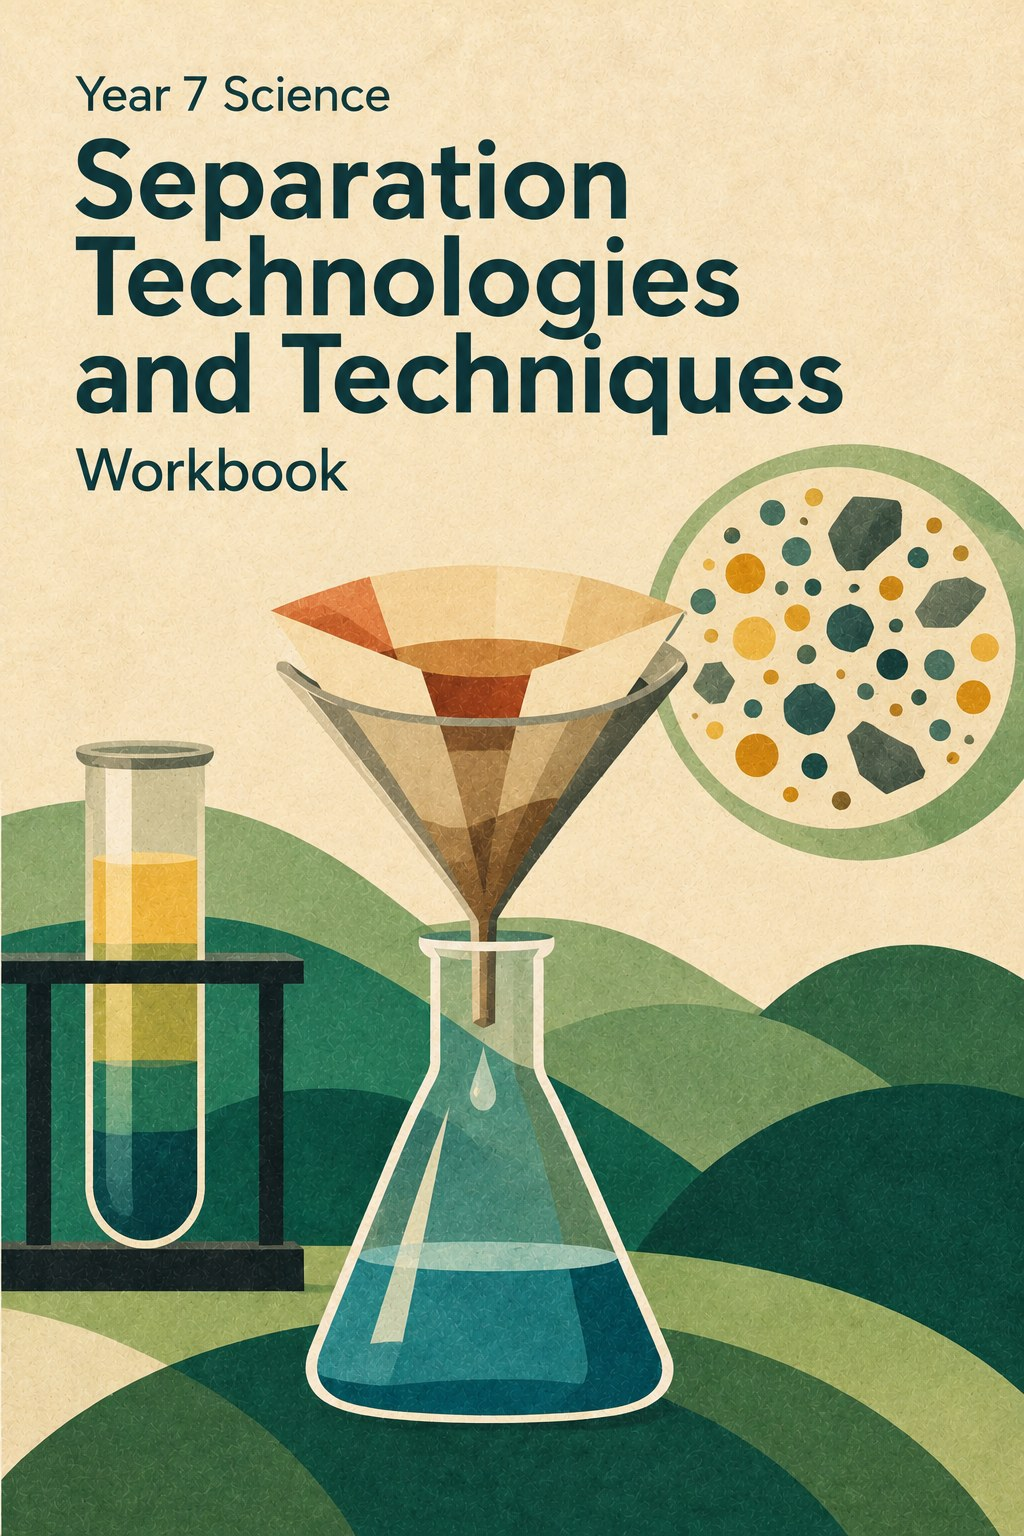
\includegraphics[width=\paperwidth]{../../../covers/separation.jpg}};
  \node[anchor=north east, fill=white, draw=Ink, line width=0.6pt, rounded corners=1.2mm,
        inner xsep=2mm, inner ysep=1.8mm, text width=30mm, font=\headingfont\footnotesize]
    at ([xshift=-4mm, yshift=-4mm]current page.north east)
    {\textbf{Name}\par\vspace{4mm}\hrule\vspace{2mm}\textbf{Class}\par\vspace{4mm}\hrule};
  \node[anchor=south east, fill=white, draw=Ink, line width=0.6pt, rounded corners=1.2mm,
        inner xsep=2.6mm, inner ysep=2mm, font=\headingfont\bfseries, align=right]
    at ([xshift=-4mm, yshift=6mm]current page.south east)
    {Lesson Booklet 1\\[-1pt]{\normalfont\headingfont\scriptsize Lessons 1--7}};
\end{tikzpicture}
\mbox{}
\clearpage

% ---- Inside cover ---------------------------------------------------------
\thispagestyle{plain}
{\headingfont\bfseries\fontsize{16}{20}\selectfont Separation Technologies and Techniques}\par\vspace{1mm}
{\headingfont\large Lesson Booklet 1 \textbullet\ Lessons 1--7 \textbullet\ Year 7}\par\vspace{1mm}
{\small\itshape VC 2.0: VC2S8U05 \textbullet\ VC2S8U06 \textbullet\ VC2S8U07 \textbullet\ VC2S8I01--I08 \textbullet\ VC2S8H02}\par\vspace{4mm}
\textbf{Teacher}\ \hrulefill\par

\begin{countrybox}{Acknowledgement of Country}
This booklet was created on the unceded Country of the Wurundjeri Woi-wurrung people of the Kulin Nation. We acknowledge Elders past, present and emerging.
\end{countrybox}

\begin{infobox}{How this booklet works}
One section for each lesson. Each opens with its key vocabulary, then:\par\smallskip
\renewcommand{\arraystretch}{1.25}
\begin{tabular}{@{}p{24mm}p{70mm}@{}}
\textbf{Part A} & a reading with comprehension questions \\
\textbf{Part B} & the ideas, worked through \\
\textbf{Part C} & practice on your own \\
\end{tabular}

\smallskip
\begin{tabular}{@{}p{24mm}p{70mm}@{}}
\textbf{I do} \tagicon{\icodots{1}} & your teacher works an example (solid frame) \\
\textbf{We do} \tagicon{\icodots{2}} & you try one together (dashed frame) \\
\textbf{Reading} \tagicon{\icoread} & a passage to read (thin frame) \\
\end{tabular}

\smallskip
Two lesson books. The experiments are in the \textbf{Experiment Booklet}. Finished your lesson work and want to go further? Ask your teacher about \textbf{Advanced Separation}.
\end{infobox}

\clearpage
\markboth{Contents}{Contents}
{\headingfont\bfseries\LARGE Contents}\par\vspace{1mm}\noindent\rule{\linewidth}{0.6pt}\par\vspace{2mm}
\renewcommand{\arraystretch}{1.45}
\begin{tabular}{|C{1.1cm}|L{6.0cm}|C{2.4cm}|}
  \hline\thead{Lesson} & \thead{Title} & \thead{Page} \\ \hline
  1 & \hyperlink{lesson.1.1}{Pure Substances} & \hyperlink{lesson.1.1}{p.\ \pageref{sec:16}} \\ \hline
  2 & \hyperlink{lesson.2.1}{Mixtures} & \hyperlink{lesson.2.1}{p.\ \pageref{sec:17}} \\ \hline
  3 & \textit{Experiment 1 --- Solubility} & Experiment Booklet \\ \hline
  4 & \hyperlink{lesson.4.1}{Classifying With Particle Diagrams} & \hyperlink{lesson.4.1}{p.\ \pageref{sec:18}} \\ \hline
  5 & \hyperlink{lesson.5.1}{Solute, Solvent and Solution} & \hyperlink{lesson.5.1}{p.\ \pageref{sec:19}} \\ \hline
  6 & \textit{Experiment 2 --- Surface Area and Dissolving} & Experiment Booklet \\ \hline
  7 & \hyperlink{lesson.7.1}{Decanting, Filtration and Magnetic Separation} & \hyperlink{lesson.7.1}{p.\ \pageref{sec:25}} \\ \hline
  8 & Evaporation and Crystallisation & Book 2 \\ \hline
  9 & \textit{Experiment 3 --- Fast and Slow Evaporation} & Experiment Booklet \\ \hline
  10 & Solubility and Saturation & Book 2 \\ \hline
  11 & \textit{Experiment 4 --- Rates of Evaporation} & Experiment Booklet \\ \hline
  12 & Solubility Curves & Book 2 \\ \hline
  13 & \textit{Experiment 5 --- Solubility and Temperature} & Experiment Booklet \\ \hline
  14 & \textit{Experiment 6 --- Growing Copper Sulfate Crystals (stretch)} & Experiment Booklet \\ \hline
  15 & \textit{Experiment 7 --- Filtration} & Experiment Booklet \\ \hline
  16 & Distillation and Chromatography & Book 2 \\ \hline
  17 & \textit{Experiment 8 --- Distillation} & Experiment Booklet \\ \hline
  18 & \textit{Experiment 9 --- The Great Green Mix Up} & Experiment Booklet \\ \hline
  --- & \hyperlink{glossary}{Glossary} & \hyperlink{glossary}{\pageref{sec:glossary}} \\ \hline
\end{tabular}
\renewcommand{\arraystretch}{1}
\clearpage
\setcounter{section}{0}\renewcommand{\lessonart}{16}
% ══════════════════════════════════════════════════════════════════════════════
%  LESSON 16 — PURE SUBSTANCES                                      (Week 6 · P1)
% ══════════════════════════════════════════════════════════════════════════════
\sectiondiv{Pure Substances}{What ``pure'' means in science \textbullet{} Pure substances in particle diagrams \textbullet{} Testing purity with melting and boiling points}\label{sec:16}
\lessoncodes{VC2S8U06}

\vocabhead
\begin{ctab}
\begin{tabular}{|SW{2.91cm}|W{8.05cm}|}
  \hd & \thead{Word} & \thead{Definition (copy from the slide)} \\ \hline
  & \scaf{\textbf{Pure substance}\label{voc:pure-substance}} & \scaf{A substance made of only one kind of particle.} \\ \hline
  & \textbf{Impure}\label{voc:impure} & \\ \hline
  & \textbf{Element}\label{voc:element} & \\ \hline
  & \textbf{Compound}\label{voc:compound} & \\ \hline
  & \textbf{Molecule}\label{voc:molecule} & \\ \hline
  & \textbf{Sample}\label{voc:sample} & \\ \hline
\end{tabular}
\end{ctab}

% ─── PART A ───────────────────────────────────────────────────────────────────
\lessonpart{A}{Reading and comprehension}{Teal}\label{read:16}

\begin{readingbox}{Reading --- Is Your Orange Juice Pure?}
A juice bottle says ``100\% pure orange juice''. To a shopper, that means nothing has been added. To a scientist, the juice is not pure at all. It is a mix of water, sugars, acids, vitamins, colours and many other substances. In science, a \textbf{pure substance} is made of only one kind of particle. Anything with more than one kind of particle mixed together is \textbf{impure}.

Pure substances are rarer than you might think. Distilled water is pure: every particle in it is a water particle. A gold bar that is 99.99\% gold is very nearly pure. Table sugar and table salt are pure substances. Tap water, air, milk, sea water and soil are not --- each contains several different kinds of particle.

A pure substance has fixed properties. Every \textbf{sample} of pure water, wherever it comes from, freezes at 0\,\textdegree C and boils at 100\,\textdegree C at sea level. Scientists use this to test purity: if a sample melts or boils at exactly the right temperature, it is probably pure. If something is mixed in, the melting and boiling points change.

The particles of a pure substance can be simple or complicated. In an \textbf{element}, like gold or oxygen, the particles are made of only one kind of atom. In a \textbf{compound}, like water or sugar, each particle is a \textbf{molecule}: a small group of different atoms joined together. But either way, if every particle in the sample is the same, the substance is pure.
\end{readingbox}

\rcreset
\rcq{Why is ``100\% pure orange juice'' not pure in the scientific sense?}{1.8cm}
\rcq{Use the passage to write a definition of a pure substance.}{1.6cm}
\rcq{List two pure substances and two impure substances from the passage.}{1.8cm}
\rcq{What does it mean that a pure substance has fixed properties?}{1.6cm}
\rcq{How can scientists use melting or boiling points to test purity?}{1.8cm}
\rcq{What is the difference between an element and a compound?}{1.8cm}
\rcq{What is a molecule?}{1.4cm}
\rcq{Water is made of two kinds of atom. Explain why it is still a pure substance.}{1.8cm}

% ─── PART B ───────────────────────────────────────────────────────────────────
\lessonpart{B}{Theory and examples}{Blue}\label{theory:16}

\subsection{What ``Pure'' Means in Science}\label{sub:16.1}

\begin{infobox}{Pure or impure?}
\textbf{Pure substance:} only \textbf{one kind} of particle, so every part of the sample is the same. \\
\textbf{Impure substance (a mixture):} \textbf{two or more kinds} of particle, mixed together.
\end{infobox}

\begin{workedex}{Pure in science, or pure in everyday speech?}
A bottle of spring water is labelled ``pure''. Is it a pure substance? Explain.

\medskip
Spring water contains dissolved minerals, such as calcium and magnesium, as well as water particles. It has \textbf{more than one kind of particle}, so it is \textbf{not a pure substance}. ``Pure'' on the label means clean and safe to drink.
\end{workedex}

\begin{wedo}{Pure in science, or pure in everyday speech?}
A jar is labelled ``pure honey''. Honey is made of water and several different sugars. Is it a pure substance? Explain.
\answerbox{2.6cm}
\end{wedo}

\subsection{Pure Substances in Particle Diagrams}\label{sub:16.2}

In a particle diagram of a pure substance, \textbf{every particle is the same}. A particle can be a single atom or a group of atoms joined together; what matters is that they are all alike.

\begin{center}
\pboxfig{\pkinds{A,A,A,A,A,A,A,A}}{A: pure}\hspace{8mm}%
\pboxfig{\pkinds{AB,AB,AB,AB,AB,AB,AB,AB}}{B: pure}\hspace{8mm}%
\pboxfig{\pkinds{A,AB,A,B,AB,A,B,AB}}{C: not pure}
\end{center}
\figcap{A and B each contain only one kind of particle. C contains three kinds.}

\begin{workedex}{Reading a particle diagram}
Explain why diagram B is a pure substance, even though each particle is made of two different atoms.

\medskip
Every particle in B is \textbf{the same}: one blue atom joined to one red atom. There is only \textbf{one kind of particle}, so B is pure. (B is a compound; A is an element.)
\end{workedex}

\begin{wedo}{Reading a particle diagram}
Explain why diagram C is not a pure substance.
\par\smallskip
\begin{center}\pboxfig{\pkinds{A,AB,A,B,AB,A,B,AB}}{C}\end{center}
\answerbox{3.0cm}
\end{wedo}

\subsection{Testing Purity}\label{sub:16.3}

\begin{workedex}{Using a boiling point}
A clear liquid boils at 100\,\textdegree C at sea level. A second clear liquid starts boiling at 102\,\textdegree C. Which one could be pure water?

\medskip
Pure water boils at exactly \textbf{100\,\textdegree C} at sea level, so the \textbf{first liquid} could be pure water. The second has something dissolved in it (salt, for example), which raises its boiling point, so it is \textbf{impure}.
\end{workedex}

\begin{wedo}{Using a melting point}
Pure lauric acid melts at 44\,\textdegree C. A sample from an old bottle melts gradually between 38\,\textdegree C and 42\,\textdegree C. Is the sample pure? Explain.
\answerbox{2.8cm}
\end{wedo}

% ─── PART C ───────────────────────────────────────────────────────────────────
\lessonpart{C}{Practice}{Amber}\label{prac:16}

Work through every task. Remember: pure means one kind of particle.

\needspace{14\baselineskip}
\task Write \textbf{PURE} or \textbf{IMPURE} for each.

\vspace{4pt}
\begin{ctab}
\begin{tabular}{|SW{3.60cm}|Z{1.46cm}|W{3.60cm}|Z{1.46cm}|}
  \hd & \thead{Material} & \thead{Pure or impure?} & \thead{Material} & \thead{Pure or impure?} \\ \hline
  & Distilled water & \scaf{PURE} & Sea water & \scaf{IMPURE} \\ \hline
  & Air & & Table sugar & \\ \hline
  & Milk & & Oxygen gas & \\ \hline
  & A 24-carat gold nugget & & Orange juice & \\ \hline
\end{tabular}
\end{ctab}

\needspace{12\baselineskip}
\task For each diagram, write \textbf{pure} or \textbf{not pure}.

\vspace{4pt}
\begin{center}
\pboxfig{\pkinds{BB,BB,BB,BB,BB,BB,BB,BB}}{P}\hspace{6mm}%
\pboxfig{\pkinds{B,B,C,B,C,B,C,B}}{Q}\hspace{6mm}%
\pboxfig{\pkinds{BAB,BAB,BAB,BAB,BAB,BAB,BAB,BAB}}{R}\hspace{6mm}%
\pboxfig{\pkinds{AA,BB,AA,BB,AA,BB,AA,BB}}{S}
\end{center}
\begin{ctab}
\begin{tabular}{|SZ{2.53cm}|Z{2.53cm}|Z{2.53cm}|Z{2.53cm}|}
  \hd & \thead{P} & \thead{Q} & \thead{R} & \thead{S} \\ \hline
  & & & & \\ \hline
\end{tabular}
\end{ctab}

\taskpair{Explain why tap water is not a pure substance.}{2.6cm}
         {Explain why salt is a pure substance but salty water is not.}{2.6cm}

\needspace{10\baselineskip}
\task A shop sells ``pure mountain air'' in cans. Is the air inside a pure substance? Explain.
\answerbox{2.6cm}

\needspace{10\baselineskip}
\task Three samples of a white powder are tested. Pure sugar melts at 186\,\textdegree C. Sample X melts at 186\,\textdegree C. Sample Y melts between 160\,\textdegree C and 175\,\textdegree C. Sample Z melts at 186\,\textdegree C.
\pt{a}Which samples could be pure sugar?
\answerbox{1.6cm}
\pt{b}Explain your answer for sample Y.
\answerbox{2.0cm}
\newpage

\newpage
\setcounter{section}{1}\renewcommand{\lessonart}{17}
% ══════════════════════════════════════════════════════════════════════════════
%  LESSON 17 — MIXTURES                                             (Week 6 · P2)
% ══════════════════════════════════════════════════════════════════════════════
\sectiondiv{Mixtures}{What a mixture is \textbullet{} Uniform and non-uniform mixtures \textbullet{} Mixtures in particle diagrams \textbullet{} Why mixtures can be separated}\label{sec:17}
\lessoncodes{VC2S8U06}

\vocabhead
\begin{ctab}
\begin{tabular}{|SW{2.91cm}|W{8.05cm}|}
  \hd & \thead{Word} & \thead{Definition (copy from the slide)} \\ \hline
  & \scaf{\textbf{Mixture}\label{voc:mixture}} & \scaf{Two or more substances mixed together but not joined, so they can be separated.} \\ \hline
  & \textbf{Uniform mixture}\label{voc:uniform-mixture} & \\ \hline
  & \textbf{Non-uniform mixture}\label{voc:non-uniform-mixture} & \\ \hline
  & \textbf{Component}\label{voc:component} & \\ \hline
  & \textbf{Separate}\label{voc:separate} & \\ \hline
  & \textbf{Suspension}\label{voc:suspension} & \\ \hline
\end{tabular}
\end{ctab}

% ─── PART A ───────────────────────────────────────────────────────────────────
\lessonpart{A}{Reading and comprehension}{Teal}\label{read:17}

\begin{readingbox}{Reading --- A World of Mixtures}
Almost everything around you is a \textbf{mixture}: two or more substances mixed together but not joined to each other. Air is a mixture of nitrogen, oxygen, argon, carbon dioxide and water vapour. Sea water is a mixture of water and salts. A muesli bar, a garden bed and the concrete of the footpath are all mixtures. Each substance in a mixture is called a \textbf{component}.

Some mixtures look the same all the way through, even under a microscope. These are \textbf{uniform mixtures}. Salt water and air are uniform: every spoonful of the sea, and every breath of air, has the same make-up. Other mixtures are \textbf{non-uniform}: you can see the different parts, and one sample can be different from another. A fruit salad is non-uniform, and so is muddy water. Muddy water is a \textbf{suspension}: tiny solid bits are spread through the liquid, but if you leave it alone they slowly sink to the bottom.

Because the components of a mixture are not joined, each one keeps its own properties. Salt water tastes salty, because the salt is still salt. Iron filings mixed with sand are still attracted to a magnet. This is the key to the last part of this unit: since each component keeps its properties, you can use those properties to \textbf{separate} a mixture into its parts.
\end{readingbox}

\rcreset
\rcq{Use the passage to write a definition of a mixture.}{1.6cm}
\rcq{Name three components of air.}{1.4cm}
\rcq{What is a component?}{1.4cm}
\rcq{What is the difference between a uniform and a non-uniform mixture?}{1.8cm}
\rcq{Give one uniform and one non-uniform mixture from the passage.}{1.6cm}
\rcq{What is a suspension? What happens if you leave one alone?}{1.8cm}
\rcq{How do you know the salt in salt water is still salt?}{1.6cm}
\rcq{Why does each component keeping its own properties make separation possible?}{1.8cm}

% ─── PART B ───────────────────────────────────────────────────────────────────
\lessonpart{B}{Theory and examples}{Blue}\label{theory:17}

\subsection{Uniform and Non-uniform Mixtures}\label{sub:17.1}

\begin{ctab}
\begin{tabular}{|L{2.39cm}|L{4.08cm}|L{4.08cm}|}
  \thead{} & \thead{Uniform mixture} & \thead{Non-uniform mixture} \\ \hline
  What you see & looks the same all the way through & you can see different parts \\ \hline
  Every sample & the same make-up & can be different \\ \hline
  Examples & salt water, air, cordial, vinegar, stainless steel & fruit salad, muddy water, sand and gravel, pizza \\ \hline
\end{tabular}
\end{ctab}

\begin{workedex}{Uniform or non-uniform?}
Is a glass of orange cordial uniform or non-uniform? Is a glass of orange juice with pulp? Explain each.

\medskip
\textbf{Cordial:} it looks the same all the way through and every sip tastes the same --- \textbf{uniform}.

\textbf{Juice with pulp:} you can see bits of pulp, and the bottom of the glass has more pulp than the top --- \textbf{non-uniform}.
\end{workedex}

\begin{wedo}{Uniform or non-uniform?}
Decide whether each mixture is uniform or non-uniform, and give a reason.
\pt{a}A bowl of breakfast cereal with milk.
\answerbox{1.6cm}
\pt{b}A glass of fizzy lemonade (ignore the bubbles).
\answerbox{1.6cm}
\end{wedo}

\subsection{Mixtures in Particle Diagrams}\label{sub:17.2}

In a particle diagram of a mixture, there are \textbf{two or more kinds of particle}, and they are \textbf{not joined} to each other.

\begin{center}
\pboxfig{\pkinds{A,B,A,A,B,A,B,A}}{a mixture of two elements}\hspace{1cm}%
\pboxfig{\pkinds{AB,AB,AB,AB,AB,AB,AB,AB}}{one compound (pure)}
\end{center}

\begin{workedex}{Mixture or compound?}
Both diagrams above contain blue and red atoms. Explain why the left one is a mixture but the right one is not.

\medskip
\textbf{Left:} the blue and red particles are \textbf{separate}, so there are two kinds of particle --- a \textbf{mixture}.

\textbf{Right:} every particle is the same blue--red pair, joined together. There is only one kind of particle, so it is a \textbf{pure substance}.
\end{workedex}

\begin{wedo}{Mixture or compound?}
Is this diagram a mixture or a pure substance? Explain.
\par\smallskip
\begin{center}\pboxfig{\pkinds{AB,AB,BB,AB,BB,AB,BB,AB}}{}\end{center}
\answerbox{3.0cm}
\end{wedo}

\subsection{Mixtures Keep Their Properties}\label{sub:17.3}

\begin{workedex}{Using properties}
Iron filings are mixed with sand. Give one property of each component that is still there in the mixture, and say how it could help separate them.

\medskip
\textbf{Iron:} is attracted to a magnet. \textbf{Sand:} is not. Running a magnet over the mixture would pull out the iron and leave the sand.
\end{workedex}

\begin{wedo}{Using properties}
Sugar is mixed with sand. Give one property of each component that is different, and suggest how it could help separate them.
\answerbox{3.0cm}
\end{wedo}

% ─── PART C ───────────────────────────────────────────────────────────────────
\lessonpart{C}{Practice}{Amber}\label{prac:17}

Work through every task. Use the words \emph{component}, \emph{uniform} and \emph{non-uniform}.

\needspace{14\baselineskip}
\task Write \textbf{U} for uniform or \textbf{N} for non-uniform.

\vspace{4pt}
\begin{ctab}
\begin{tabular}{|SW{3.78cm}|Z{1.28cm}|W{3.78cm}|Z{1.28cm}|}
  \hd & \thead{Mixture} & \thead{U or N?} & \thead{Mixture} & \thead{U or N?} \\ \hline
  & Salt water & \scaf{U} & Sand and water & \scaf{N} \\ \hline
  & Trail mix & & Vinegar & \\ \hline
  & Air in a room & & A bowl of soup with vegetables & \\ \hline
  & Muddy water & & Black coffee & \\ \hline
\end{tabular}
\end{ctab}

\needspace{12\baselineskip}
\task Name the components of each mixture.

\vspace{4pt}
\begin{ctab}
\begin{tabular}{|SW{2.96cm}|W{8.00cm}|}
  \hd & \thead{Mixture} & \thead{Components} \\ \hline
  & \scaf{Salt water} & \scaf{salt and water} \\ \hline
  & Cordial & \\ \hline
  & A cup of tea with milk and sugar & \\ \hline
  & Sand and gravel & \\ \hline
\end{tabular}
\end{ctab}

\taskpair{Explain why air is a mixture, not a pure substance.}{2.6cm}
         {Explain why muddy water is called a suspension.}{2.6cm}

\needspace{10\baselineskip}
\task Ruby says, ``Salt water is a pure substance because it looks the same all the way through.'' Explain why Ruby is wrong.
\answerbox{2.8cm}

\needspace{12\baselineskip}
\task Draw a particle diagram of a mixture of two different gases. Use two kinds of circles, and label what each one is.
\drawbox{5cm}{}
\newpage

\newpage
\setcounter{section}{3}\renewcommand{\lessonart}{18}
% ══════════════════════════════════════════════════════════════════════════════
%  LESSON 18 — CLASSIFYING WITH PARTICLE DIAGRAMS                   (Week 6 · P3)
% ══════════════════════════════════════════════════════════════════════════════
\sectiondiv{Classifying With Particle Diagrams}{A classification flowchart \textbullet{} Pure or mixture? \textbullet{} Which state? \textbullet{} Drawing your own diagrams}\label{sec:18}
\lessoncodes{VC2S8U05 \textbullet{} VC2S8U06}

\vocabhead
\begin{ctab}
\begin{tabular}{|SW{2.91cm}|W{8.05cm}|}
  \hd & \thead{Word} & \thead{Definition (copy from the slide)} \\ \hline
  & \scaf{\textbf{Classify}\label{voc:classify}} & \scaf{To sort things into groups using what they have in common.} \\ \hline
  & \textbf{Flowchart}\label{voc:flowchart} & \\ \hline
  & \textbf{Key}\label{voc:key} & \\ \hline
  & \textbf{Criteria}\label{voc:criteria} & \\ \hline
  & \textbf{Justify}\label{voc:justify} & \\ \hline
  & \textbf{Represent}\label{voc:represent} & \\ \hline
\end{tabular}
\end{ctab}

% ─── PART A ───────────────────────────────────────────────────────────────────
\lessonpart{A}{Reading and comprehension}{Teal}\label{read:18}

\begin{readingbox}{Reading --- Sorting the Invisible}
Scientists love to \textbf{classify}: to sort things into groups so they can see patterns. Biologists sort living things into kingdoms and species. Chemists sort matter. And because the particles that matter is made of are far too small to see, chemists often sort it using particle diagrams, which \textbf{represent} the particles as circles.

To classify, you need clear \textbf{criteria}: the questions you ask to decide which group something belongs in. For matter, two questions do almost all the work. First: how many kinds of particle are there? One kind means a pure substance; two or more means a mixture. Second: how are the particles arranged? Packed in a pattern means a solid; close together but jumbled means a liquid; far apart means a gas.

A \textbf{flowchart} puts the criteria in order, so you answer one question at a time and follow the arrows to the answer. Every particle diagram also needs a \textbf{key}: a small table that shows what each kind of circle stands for. Without a key, a red circle could mean anything.

Finally, a good scientist does not just give an answer, but can \textbf{justify} it: give the evidence from the diagram that supports the answer. ``It's a mixture'' is an answer. ``It's a mixture because it has two kinds of particle that are not joined'' is a justified answer.
\end{readingbox}

\rcreset
\rcq{What does it mean to classify?}{1.4cm}
\rcq{Why do chemists use particle diagrams to classify matter?}{1.6cm}
\rcq{What are criteria?}{1.4cm}
\rcq{What two questions does the passage say do almost all the work?}{1.8cm}
\rcq{How does the arrangement of particles tell you the state?}{1.8cm}
\rcq{What does a flowchart do?}{1.4cm}
\rcq{Why does every particle diagram need a key?}{1.6cm}
\rcq{What is the difference between giving an answer and justifying it?}{1.8cm}

% ─── PART B ───────────────────────────────────────────────────────────────────
\lessonpart{B}{Theory and examples}{Blue}\label{theory:18}

\subsection{A Classification Flowchart}\label{sub:18.1}

\begin{center}
\begin{fitbox}\begin{tikzpicture}[font=\small, every node/.style={align=center},
  q/.style={draw=NavyBlue, fill=LightBlue, rounded corners, minimum width=4.2cm, minimum height=0.9cm},
  a/.style={draw=GoldDark, fill=GoldLight, rounded corners, minimum width=3.0cm, minimum height=0.8cm, font=\small\bfseries}]
  \node[q] (q1) at (0,0) {How many kinds of\\particle are there?};
  \node[a] (pure) at (-3.6,-1.8) {PURE\\SUBSTANCE};
  \node[a] (mix) at (3.6,-1.8) {MIXTURE};
  \draw[thin arrow] (q1) -- node[left, font=\scriptsize] {one\ } (pure);
  \draw[thin arrow] (q1) -- node[right, font=\scriptsize] {\ two or more} (mix);
  \node[q] (q2) at (0,-3.6) {How are the particles\\arranged?};
  \draw[thin arrow] (pure) |- (q2);
  \draw[thin arrow] (mix) |- (q2);
  \node[a] (s) at (-4.2,-5.4) {SOLID};
  \node[a] (l) at (0,-5.4) {LIQUID};
  \node[a] (g) at (4.2,-5.4) {GAS};
  \draw[thin arrow] (q2) -- node[left, font=\scriptsize] {touching,\\in a pattern\ } (s);
  \draw[thin arrow] (q2) -- node[right, font=\scriptsize] {touching,\\jumbled} (l);
  \draw[thin arrow] (q2) -- node[right, font=\scriptsize] {\ far apart} (g);
\end{tikzpicture}\end{fitbox}
\end{center}
\figcap{Two questions classify almost any particle diagram.}

\begin{workedex}{Using the flowchart}
Classify this diagram. Justify your answer.
\begin{center}\pboxfig{\pkinds{A,BB,A,BB,A,BB,A,BB}}{}\end{center}

\textbf{Kinds of particle:} two --- single blue atoms and red pairs, not joined to each other. So it is a \textbf{mixture}.

\textbf{Arrangement:} far apart, spread through the box. So it is a \textbf{gas}.

\medskip
\textbf{A mixture of two gases.}
\end{workedex}

\begin{wedo}{Using the flowchart}
Classify this diagram, and justify your answer.
\par\smallskip
\begin{center}\pboxfig{\stateIn{solid}{pC}}{}\end{center}
\pt{a}Pure or mixture? Why?
\answerbox{1.6cm}
\pt{b}Which state? Why?
\answerbox{1.6cm}
\end{wedo}

\subsection{Liquids and Solids That Are Mixtures}\label{sub:18.2}

\begin{workedex}{A liquid mixture}
Classify this diagram, and justify your answer.
\begin{center}\begin{fitbox}\begin{tikzpicture}\foreach \x/\y [count=\i] in {2.29/0.20,0.42/0.20,1.28/0.20,0.85/0.20,1.87/0.20,1.07/0.47,1.45/0.49,0.28/0.51,0.72/0.52,2.34/0.54,1.87/0.54,1.29/0.80,2.03/0.85,0.27/0.86,0.69/0.86,1.68/0.90,2.34/0.98,0.88/1.15,2.01/1.20,1.63/1.24,0.55/1.26,1.18/1.31,2.36/1.33,0.23/1.39,0.88/1.50,1.99/1.55,1.65/1.59,0.51/1.61,1.30/1.63}{\ifodd\i\node[pA] at (\x,\y) {};\else\ifnum\i<14\node[pB] at (\x,\y) {};\else\node[pA] at (\x,\y) {};\fi\fi}\pbox\end{tikzpicture}\end{fitbox}\end{center}

\textbf{Kinds of particle:} two (blue and red), not joined --- a \textbf{mixture}.

\textbf{Arrangement:} touching but jumbled --- a \textbf{liquid}. \quad \textbf{A liquid mixture}, such as a solution.
\end{workedex}

\begin{wedo}{A solid mixture}
Draw a particle diagram of a solid mixture of two metals. Include a key.
\drawbox{4.6cm}{}
\end{wedo}

% ─── PART C ───────────────────────────────────────────────────────────────────
\lessonpart{C}{Practice}{Amber}\label{prac:18}

Work through every task. Classify each diagram as pure or mixture, and as solid, liquid or gas.

\needspace{20\baselineskip}
\task Classify each diagram.

\vspace{4pt}
\begin{center}
\pboxfig{\pkinds{AA,AA,AA,AA,AA,AA,AA,AA}}{1}\hspace{5mm}%
\pboxfig{\stateIn{liquid}{pD}}{2}\hspace{5mm}%
\pboxfig{\pkinds{A,C,AB,A,C,AB,A,C}}{3}\hspace{5mm}%
\pboxfig{\foreach \r in {0,...,4}{\foreach \c in {0,...,6}{\pgfmathtruncatemacro\k{mod(\r+\c,2)}\ifnum\k=0\node[pB] at (0.31+\c*0.33,0.2+\r*0.33) {};\else\node[pC] at (0.31+\c*0.33,0.2+\r*0.33) {};\fi}}}{4}
\end{center}
\begin{ctab}
\begin{tabular}{|SZ{1.09cm}|Z{3.01cm}|Z{3.01cm}|W{3.01cm}|}
  \hd & \thead{Diagram} & \thead{Pure or mixture?} & \thead{State} & \thead{Evidence} \\ \hline
  & \scaf{1} & \scaf{pure} & \scaf{gas} & \scaf{one kind of particle, far apart} \\ \hline
  & 2 & & & \\ \hline
  & 3 & & & \\ \hline
  & 4 & & & \\ \hline
\end{tabular}
\end{ctab}

\needspace{12\baselineskip}
\task Draw a particle diagram of a pure liquid. Include a key.
\drawbox{4.6cm}{}

\needspace{12\baselineskip}
\task Draw a particle diagram of a mixture of a gas and a solid, such as dust in air. Include a key.
\drawbox{4.6cm}{}

\needspace{10\baselineskip}
\task Ben says, ``This diagram is a mixture because it has blue and red atoms.'' The diagram shows eight identical particles, each made of one blue atom joined to one red atom. Explain why Ben is wrong.
\answerbox{2.8cm}

\needspace{10\baselineskip}
\task A diagram shows particles that are touching and arranged in a regular pattern, with two different colours of particle that are not joined. Classify it, and give an everyday example of a material it could represent.
\answerbox{2.6cm}
\newpage

\newpage
\setcounter{section}{4}\renewcommand{\lessonart}{19}
% ══════════════════════════════════════════════════════════════════════════════
%  LESSON 19 — SOLUTE, SOLVENT AND SOLUTION                         (Week 7 · P1)
% ══════════════════════════════════════════════════════════════════════════════
\sectiondiv{Solute, Solvent and Solution}{Dissolving with particles \textbullet{} Soluble and insoluble \textbullet{} Mass is conserved \textbullet{} Concentrated and dilute}\label{sec:19}
\lessoncodes{VC2S8U06 \textbullet{} VC2S8U05}

\vocabhead
\begin{ctab}
\begin{tabular}{|SW{2.91cm}|W{8.05cm}|}
  \hd & \thead{Word} & \thead{Definition (copy from the slide)} \\ \hline
  & \scaf{\textbf{Solution}\label{voc:solution}} & \scaf{A uniform mixture made when a substance dissolves in a liquid.} \\ \hline
  & \textbf{Solute}\label{voc:solute} & \\ \hline
  & \textbf{Solvent}\label{voc:solvent} & \\ \hline
  & \textbf{Dissolve}\label{voc:dissolve} & \\ \hline
  & \textbf{Soluble}\label{voc:soluble} & \\ \hline
  & \textbf{Insoluble}\label{voc:insoluble} & \\ \hline
\end{tabular}
\end{ctab}

% ─── PART A ───────────────────────────────────────────────────────────────────
\lessonpart{A}{Reading and comprehension}{Teal}\label{read:19}

\begin{readingbox}{Reading --- Where Does the Sugar Go?}
Stir a spoonful of sugar into a cup of tea and it seems to vanish. But taste the tea and you know the sugar is still there. It has not disappeared; it has \textbf{dissolved}. The sugar particles have separated from each other and spread out evenly between the water particles, far too small to see. The sweet tea is a \textbf{solution}: a uniform mixture.

Every solution has two parts. The \textbf{solute} is the substance that dissolves --- here, the sugar. The \textbf{solvent} is the liquid it dissolves in --- here, the water in the tea. Water dissolves so many substances that it is sometimes called the universal solvent, but it cannot dissolve everything.

A substance that dissolves in a solvent is \textbf{soluble} in it. Sugar, salt and instant coffee are soluble in water. A substance that does not dissolve is \textbf{insoluble}. Sand, chalk and pepper are insoluble in water: stir them in and they just swirl around, then settle to the bottom. Whether something is soluble depends on the solvent, too. Nail polish is insoluble in water, which is why washing your hands will not remove it, but it dissolves in acetone, the solvent in nail polish remover.

People often say that sugar ``melts'' in tea. It does not. Melting needs only heat, and changes a solid to a liquid on its own. Dissolving needs a solvent, and works perfectly well in cold water too.
\end{readingbox}

\rcreset
\rcq{How do you know the sugar is still in the tea after it seems to vanish?}{1.6cm}
\rcq{Describe what the sugar particles do when sugar dissolves.}{1.8cm}
\rcq{In sweet tea, what is the solute and what is the solvent?}{1.4cm}
\rcq{What is the difference between soluble and insoluble?}{1.6cm}
\rcq{Give two substances that are soluble in water and two that are insoluble.}{1.6cm}
\rcq{Why does washing your hands not remove nail polish?}{1.6cm}
\rcq{What does it mean that solubility ``depends on the solvent''?}{1.6cm}
\rcq{Explain why sugar dissolving in tea is not melting.}{1.8cm}

% ─── PART B ───────────────────────────────────────────────────────────────────
\lessonpart{B}{Theory and examples}{Blue}\label{theory:19}

\subsection{Dissolving With Particles}\label{sub:19.1}

\begin{center}\begin{fitbox}\begin{tikzpicture}[font=\small]
  \begin{scope}
    \foreach \x/\y in {2.29/0.20,0.42/0.20,1.28/0.20,0.85/0.20,1.87/0.20,1.07/0.47,1.45/0.49,0.28/0.51,0.72/0.52,2.34/0.54,1.87/0.54,1.29/0.80,2.03/0.85,0.27/0.86,0.69/0.86,1.68/0.90,2.34/0.98,0.88/1.15,2.01/1.20,1.63/1.24,0.55/1.26,1.18/1.31,2.36/1.33,0.23/1.39,0.88/1.50,1.99/1.55,1.65/1.59,0.51/1.61,1.30/1.63}{\node[pA] at (\x,\y) {};}
    \foreach \r in {0,1}{\foreach \c in {0,1,2}{\node[pC] at (0.95+\c*0.33,2.0+\r*0.33) {};}}
    \pbox \node[font=\small\bfseries, text=NavyBlue] at (1.3,-0.35) {sugar added};
  \end{scope}
  \draw[thin arrow, DarkGrey] (3.0,1.3) -- node[above, font=\scriptsize] {stir} (3.9,1.3);
  \begin{scope}[xshift=4.3cm]
    \foreach \x/\y [count=\i] in {2.29/0.20,0.42/0.20,1.28/0.20,0.85/0.20,1.87/0.20,1.07/0.47,1.45/0.49,0.28/0.51,0.72/0.52,2.34/0.54,1.87/0.54,1.29/0.80,2.03/0.85,0.27/0.86,0.69/0.86,1.68/0.90,2.34/0.98,0.88/1.15,2.01/1.20,1.63/1.24,0.55/1.26,1.18/1.31,2.36/1.33,0.23/1.39,0.88/1.50,1.99/1.55,1.65/1.59,0.51/1.61,1.30/1.63,0.75/1.85,1.7/1.88,2.25/1.7,0.3/1.8,1.25/1.95}{%
      \ifnum\i=3 \node[pC] at (\x,\y) {};\else\ifnum\i=10 \node[pC] at (\x,\y) {};\else\ifnum\i=16 \node[pC] at (\x,\y) {};\else\ifnum\i=21 \node[pC] at (\x,\y) {};\else\ifnum\i=27 \node[pC] at (\x,\y) {};\else\ifnum\i=32 \node[pC] at (\x,\y) {};\else\node[pA] at (\x,\y) {};\fi\fi\fi\fi\fi\fi}
    \pbox \node[font=\small\bfseries, text=NavyBlue] at (1.3,-0.35) {dissolved: a solution};
  \end{scope}
  \node[pC] at (8.0,1.6) {}; \node[anchor=west, lab, font=\small] at (8.2,1.6) {sugar (solute)};
  \node[pA] at (8.0,1.0) {}; \node[anchor=west, lab, font=\small] at (8.2,1.0) {water (solvent)};
\end{tikzpicture}\end{fitbox}\end{center}
\figcap{When sugar dissolves, its particles separate and spread evenly between the water particles.}

\begin{workedex}{Explaining dissolving}
Explain, using particles, what happens when salt dissolves in water.

\medskip
Water particles are attracted to the salt particles at the surface of each grain and pull them away. The salt particles \textbf{separate} from each other and \textbf{spread out evenly} between the water particles. The salt is still there, but its particles are too small and too spread out to see.
\end{workedex}

\begin{wedo}{Explaining dissolving}
A sugar cube is dropped into a glass of still water. An hour later, the cube is gone and the water tastes sweet everywhere. Explain, using particles, what happened.
\answerbox{3.0cm}
\end{wedo}

\subsection{Mass Is Conserved}\label{sub:19.2}

When a solute dissolves, no particles are lost. The mass of the solution is the mass of the solvent plus the mass of the solute.

\begin{workedex}{Mass of a solution}
10\,g of salt is dissolved in 200\,g of water. What is the mass of the solution?

\medskip
mass of solution $=$ mass of solvent $+$ mass of solute $= 200 + 10 = \mathbf{210\ g}$
\end{workedex}

\begin{wedo}{Mass of a solution}
A student dissolves 25\,g of sugar in 150\,g of water. What is the mass of the sugar solution?
\workbox{2.4cm}
\end{wedo}

\subsection{Concentrated and Dilute}\label{sub:19.3}

A \textbf{concentrated} solution has a lot of solute in a small amount of solvent; a \textbf{dilute} solution has only a little. Adding more water makes a solution more dilute.

\begin{workedex}{Comparing concentrations}
Glass A has 10\,g of sugar in 100\,mL of water. Glass B has 10\,g of sugar in 250\,mL of water. Which is more concentrated?

\medskip
Both have the same mass of solute, but A has \textbf{less solvent}. The sugar particles in A are packed more closely among the water particles, so \textbf{A is more concentrated}.
\end{workedex}

\begin{wedo}{Comparing concentrations}
Jug A holds 50\,mL of cordial mixed with 500\,mL of water. Jug B holds 50\,mL of cordial mixed with 1000\,mL of water. Which is more dilute? Explain.
\answerbox{2.4cm}
\end{wedo}

% ─── PART C ───────────────────────────────────────────────────────────────────
\lessonpart{C}{Practice}{Amber}\label{prac:19}

Work through every task. Use the words \emph{solute}, \emph{solvent} and \emph{solution} correctly.

\needspace{14\baselineskip}
\task Name the solute and the solvent in each solution.

\vspace{4pt}
\begin{ctab}
\begin{tabular}{|SW{3.71cm}|Z{3.41cm}|Z{3.41cm}|}
  \hd & \thead{Solution} & \thead{Solute} & \thead{Solvent} \\ \hline
  & \scaf{Salt water} & \scaf{salt} & \scaf{water} \\ \hline
  & Instant coffee & & \\ \hline
  & Cordial drink & & \\ \hline
  & Sea water & & \\ \hline
\end{tabular}
\end{ctab}

\needspace{12\baselineskip}
\task Write \textbf{S} if the substance is soluble in water and \textbf{I} if it is insoluble.

\vspace{4pt}
\begin{ctab}
\begin{tabular}{|SW{3.78cm}|Z{1.28cm}|W{3.78cm}|Z{1.28cm}|}
  \hd & \thead{Substance} & \thead{S or I?} & \thead{Substance} & \thead{S or I?} \\ \hline
  & Salt & \scaf{S} & Sand & \scaf{I} \\ \hline
  & Sugar & & Chalk & \\ \hline
  & Pepper & & Instant coffee & \\ \hline
\end{tabular}
\end{ctab}

\taskpair{15\,g of salt is dissolved in 250\,g of water. Find the mass of the solution.}{2.6cm}
         {A solution has a mass of 120\,g. It was made with 100\,g of water. What mass of solute was used?}{2.6cm}

\needspace{10\baselineskip}
\task Explain, using particles, why you cannot see the salt in salt water, even though it is still there.
\answerbox{2.8cm}

\needspace{10\baselineskip}
\task Ella says, ``The sugar melted in my hot chocolate.'' Explain why ``melted'' is the wrong word, and say what the right word is.
\answerbox{2.6cm}

\needspace{10\baselineskip}
\task A student stirs a spoonful of flour into water. The water goes cloudy, and after ten minutes a white layer has settled at the bottom. Is flour soluble or insoluble in water? Use the evidence to explain.
\answerbox{2.6cm}
\newpage

\newpage
\setcounter{section}{6}\renewcommand{\lessonart}{25}
% ══════════════════════════════════════════════════════════════════════════════
%  LESSON 25 — DECANTING, FILTRATION AND MAGNETIC SEPARATION        (Week 9 · P1)
% ══════════════════════════════════════════════════════════════════════════════
\sectiondiv{Decanting, Filtration and Magnetic Separation}{Choosing a technique from a property \textbullet{} Sieving and winnowing \textbullet{} Decanting \textbullet{} Filtration \textbullet{} Magnetic separation}\label{sec:25}
\lessoncodes{VC2S8U06 \textbullet{} VC2S8I03}

\vocabhead
\begin{ctab}
\begin{tabular}{|SW{2.91cm}|W{8.05cm}|}
  \hd & \thead{Word} & \thead{Definition (copy from the slide)} \\ \hline
  & \scaf{\textbf{Separation technique}\label{voc:separation-technique}} & \scaf{A method for splitting a mixture into its parts using a property that differs between them.} \\ \hline
  & \textbf{Sieving}\label{voc:sieving} & \\ \hline
  & \textbf{Decanting}\label{voc:decanting} & \\ \hline
  & \textbf{Filtration}\label{voc:filtration} & \\ \hline
  & \textbf{Residue}\label{voc:residue} & \\ \hline
  & \textbf{Filtrate}\label{voc:filtrate} & \\ \hline
\end{tabular}
\end{ctab}

% ─── PART A ───────────────────────────────────────────────────────────────────
\lessonpart{A}{Reading and comprehension}{Teal}\label{read:25}

\begin{readingbox}{Reading --- Separating by Size, Weight and Magnetism}
Every \textbf{separation technique} works the same way: find a property that is different for the parts of the mixture, then use that difference to pull them apart. The simplest property is size. \textbf{Sieving} lets small pieces fall through a mesh while big pieces stay behind. Builders sieve sand to get the stones out of it.

Aboriginal peoples in many parts of Australia have used separation techniques for tens of thousands of years. To prepare grass and wattle seeds for grinding into flour, women tossed the seeds in a shallow wooden dish called a coolamon. The heavy seeds dropped back into the dish while the light husks were caught by the breeze and carried away. This technique, called winnowing, separates by mass and size.

When a mixture of a solid and a liquid is left to stand, a heavy insoluble solid settles to the bottom. You can then carefully pour off the liquid, leaving the solid behind. This is \textbf{decanting}. It is quick, but some liquid always stays with the solid, and fine particles can slip over with the liquid.

For a cleaner result, use \textbf{filtration}. The mixture is poured through filter paper in a funnel. The paper is full of tiny holes: water and anything dissolved in it can pass through, but grains of an insoluble solid cannot. The solid trapped in the paper is the \textbf{residue}; the liquid that passes through is the \textbf{filtrate}. Coffee machines, swimming pool filters and the kidneys all use filtration.

Some metals, especially iron, are attracted to a magnet. Recycling plants use huge electromagnets to lift steel cans out of a stream of mixed rubbish, a technique called magnetic separation.
\end{readingbox}

\rcreset
\rcq{What is the first step in choosing any separation technique?}{1.6cm}
\rcq{Which property does sieving use? Give the passage's example.}{1.6cm}
\rcq{Describe how winnowing in a coolamon separates seeds from husks.}{2.0cm}
\rcq{When can a mixture be separated by decanting?}{1.6cm}
\rcq{Give one problem with decanting.}{1.4cm}
\rcq{Explain why filter paper lets water through but not sand.}{1.8cm}
\rcq{What is the difference between the residue and the filtrate?}{1.6cm}
\rcq{How do recycling plants separate steel cans from other rubbish?}{1.6cm}

% ─── PART B ───────────────────────────────────────────────────────────────────
\lessonpart{B}{Theory and examples}{Blue}\label{theory:25}

\subsection{Choosing a Technique From a Property}\label{sub:25.1}

\begin{ctab}
\begin{tabular}{|L{2.67cm}|L{3.79cm}|L{4.08cm}|}
  \thead{Technique} & \thead{Property it uses} & \thead{Example} \\ \hline
  Sieving & size of the pieces & stones out of sand \\ \hline
  Winnowing & mass and size (light pieces blow away) & husks from seeds \\ \hline
  Decanting & a heavy solid settles; the liquid pours & water off settled mud \\ \hline
  Filtration & an insoluble solid cannot pass through filter paper & sand out of water \\ \hline
  Magnetic separation & some metals are attracted to a magnet & iron filings from sulfur \\ \hline
\end{tabular}
\end{ctab}

\begin{workedex}{Choosing a technique}
A mixture contains dried peas and rice. Choose a technique to separate them and explain your choice.

\medskip
\textbf{Property that differs:} size --- peas are much bigger than grains of rice.

\textbf{Technique:} \textbf{sieving} with a mesh that the rice falls through but the peas cannot.
\end{workedex}

\begin{wedo}{Choosing a technique}
A mixture contains iron nails and wood shavings. Choose a technique to separate them, and name the property that differs.
\answerbox{2.6cm}
\end{wedo}

\subsection{Filtration}\label{sub:25.2}

\diagFiltration
\figcap{Filtration: the insoluble solid is trapped as residue; the filtrate passes through.}

\begin{workedex}{What does filtration separate?}
Sand and salt water are poured through filter paper. Which parts end up in the residue and which in the filtrate?

\medskip
\textbf{Residue:} the \textbf{sand}, because it is insoluble and its grains are too big for the holes in the paper.

\textbf{Filtrate:} the \textbf{salt water}. The salt is dissolved, so its particles are small enough to pass through with the water.
\end{workedex}

\begin{wedo}{What does filtration separate?}
Muddy water with sugar dissolved in it is filtered.
\pt{a}What is the residue?
\answerbox{1.4cm}
\pt{b}What is the filtrate? Does it taste sweet? Explain.
\answerbox{2.2cm}
\end{wedo}

\subsection{Separating in Several Steps}\label{sub:25.3}

\begin{workedex}{A multi-step separation}
A mixture contains iron filings, sand and salt. Describe how to get the sand on its own.

\medskip
\textbf{Step 1:} run a magnet over the dry mixture to remove the \textbf{iron filings}.

\textbf{Step 2:} stir the rest into water; the salt dissolves but the sand does not.

\textbf{Step 3:} \textbf{filter}. The sand is the residue; dry it on the filter paper.
\end{workedex}

\begin{wedo}{A multi-step separation}
A mixture contains small stones, sand and sugar. Describe the steps to get the sand on its own, naming each technique.
\answerbox{3.4cm}
\end{wedo}

% ─── PART C ───────────────────────────────────────────────────────────────────
\lessonpart{C}{Practice}{Amber}\label{prac:25}

Work through every task. Name the property that differs before you choose a technique.

\needspace{14\baselineskip}
\task Choose a technique to separate each mixture, and name the property it uses.

\vspace{4pt}
\begin{ctab}
\begin{tabular}{|SW{3.42cm}|Z{2.99cm}|W{4.13cm}|}
  \hd & \thead{Mixture} & \thead{Technique} & \thead{Property that differs} \\ \hline
  & \scaf{Chalk dust in water} & \scaf{filtration} & \scaf{chalk is insoluble} \\ \hline
  & Gravel and sand & & \\ \hline
  & Steel paperclips and plastic beads & & \\ \hline
  & Water above settled mud in a bucket & & \\ \hline
\end{tabular}
\end{ctab}

\taskpair{Explain why filtering salt water does not remove the salt.}{2.6cm}
         {Give one advantage of filtration over decanting.}{2.6cm}

\needspace{10\baselineskip}
\task A mixture of grass seeds and dry husks is tossed gently in a shallow wooden dish (a coolamon) in a light breeze. Explain how this separates the husks from the seeds, and name the properties that make it work.
\answerbox{2.8cm}

\needspace{10\baselineskip}
\task A student filters muddy water, but the filtrate is still slightly cloudy. Suggest two reasons why.
\answerbox{2.6cm}

\needspace{10\baselineskip}
\task A mixture contains iron filings, salt and pepper. Pepper is insoluble in water. Describe the steps to get all three back separately, naming each technique.
\answerbox{3.6cm}
\newpage

\newpage
\clearpage\markboth{Glossary}{Glossary}\hypertarget{glossary}{}\pdfbookmark[1]{Glossary}{glossarybm}
{\headingfont\bfseries\LARGE Glossary}\label{sec:glossary}\par\vspace{1mm}\noindent\rule{\linewidth}{0.6pt}\par
{\small Every key word in this booklet and the page it is introduced on.}\par\smallskip
\renewcommand{\arraystretch}{1.3}
\begin{longtable}{|>{\RaggedRight}p{34mm}|p{9mm}|p{\dimexpr\linewidth-43mm-6\tabcolsep-4\arrayrulewidth-1pt\relax}|}
\hline \rule{0pt}{4mm}\headingfont\bfseries Word & \headingfont\bfseries Page & \headingfont\bfseries In my own words \\ \hline \endhead
  Classify & \pageref{voc:classify} & \\ \hline
  Component & \pageref{voc:component} & \\ \hline
  Compound & \pageref{voc:compound} & \\ \hline
  Criteria & \pageref{voc:criteria} & \\ \hline
  Decanting & \pageref{voc:decanting} & \\ \hline
  Dissolve & \pageref{voc:dissolve} & \\ \hline
  Element & \pageref{voc:element} & \\ \hline
  Filtrate & \pageref{voc:filtrate} & \\ \hline
  Filtration & \pageref{voc:filtration} & \\ \hline
  Flowchart & \pageref{voc:flowchart} & \\ \hline
  Impure & \pageref{voc:impure} & \\ \hline
  Insoluble & \pageref{voc:insoluble} & \\ \hline
  Justify & \pageref{voc:justify} & \\ \hline
  Key & \pageref{voc:key} & \\ \hline
  Mixture & \pageref{voc:mixture} & \\ \hline
  Molecule & \pageref{voc:molecule} & \\ \hline
  Non-uniform mixture & \pageref{voc:non-uniform-mixture} & \\ \hline
  Pure substance & \pageref{voc:pure-substance} & \\ \hline
  Represent & \pageref{voc:represent} & \\ \hline
  Residue & \pageref{voc:residue} & \\ \hline
  Sample & \pageref{voc:sample} & \\ \hline
  Separate & \pageref{voc:separate} & \\ \hline
  Separation technique & \pageref{voc:separation-technique} & \\ \hline
  Sieving & \pageref{voc:sieving} & \\ \hline
  Soluble & \pageref{voc:soluble} & \\ \hline
  Solute & \pageref{voc:solute} & \\ \hline
  Solution & \pageref{voc:solution} & \\ \hline
  Solvent & \pageref{voc:solvent} & \\ \hline
  Suspension & \pageref{voc:suspension} & \\ \hline
  Uniform mixture & \pageref{voc:uniform-mixture} & \\ \hline
\end{longtable}
\padtofour
\end{document}
